% LaTeX-Vorlage Version 3.1,  Juli 2011

 
\documentclass[a4paper,bibtotoc,oneside]{scrbook} 
% F"ur kurze Arbeiten w"are auch die Dokumentklasse "scrartcl" ausreichend. In diesem Fall ist "section" die h"ochste Ebene ("chapter" gibt es dann nicht).
% \documentclass[a4paper,bibtotoc,oneside]{scrartcl}


% verlinkte Querverweise im pdf
\usepackage{hyperref}

% deutsche Anpassungen
%\usepackage[ansinew]{inputenc}
\usepackage[utf8]{inputenc}
\usepackage[T1]{fontenc}
\usepackage[ngerman]{babel}




% mathematische Symbole
\usepackage{amsmath,amssymb,amsfonts,amstext}

% Kopfzeilen frei gestaltbar
\usepackage{fancyhdr}
\lfoot[\fancyplain{}{}]{\fancyplain{}{}}
\rfoot[\fancyplain{}{}]{\fancyplain{}{}}
\cfoot[\fancyplain{}{\footnotesize\thepage}]{\fancyplain{}{\footnotesize\thepage}}
\lhead[\fancyplain{}{\footnotesize\nouppercase\leftmark}]{\fancyplain{}{}}
\chead{}
\rhead[\fancyplain{}{}]{\fancyplain{}{\footnotesize\nouppercase\sc\leftmark}} 

% Farben im Dokument m"oglich
\usepackage{color}

% Schriftart Helvetica
\usepackage{helvet}
\renewcommand{\familydefault}{cmss} 

% Graphiken einbinden: hier f"ur pdflatex
\usepackage[pdftex]{graphicx}

\usepackage{array}

\usepackage{subfigure} 

\usepackage{multirow}

% H"ohe und Breite des Textk"orpers etwas gr"osser definieren
\setlength{\textheight}{225mm}
\setlength{\textwidth}{1.05\textwidth}

% weniger Warnungen wegen "uberf"ullter Boxen
\tolerance = 9999
\sloppy

% Anpassung einiger "Uberschriften 
\renewcommand\figurename{Abbildung}
\renewcommand\tablename{Tabelle}



\begin{document}

% Kopf- und Fusszeilen initiieren
\pagestyle{fancy}

% Deckblatt:
\thispagestyle{empty}
\begin{picture}(0,0)
\color{white}\sffamily
\put(-101,-749){
\includegraphics[width=1.002\paperwidth, height=\paperheight]{img/BM_2011.pdf}}
\put(220,-670){
\includegraphics[width=0.5\textwidth]{img/FHTW_Logo_4c.pdf}}
\put(-30, -20){\bfseries\huge MASTER THESIS}
\put(-30,-50){\Large zur Erlangung des akademischen Grades}
\put(-30,-70){\Large \glqq Master of Science in Engineering\grqq}
% Titel des Studienganges einf"ugen:
\put(-30,-90){\Large im Studiengang Industrielle Elektronik}
% Titel der Arbeit einf"ugen:
% Die Minipage wird gesetzt, damit auch mehrzeilige Titel m"oglich werden.
\put(-32,-180){
\begin{minipage}{14cm}
\bfseries\huge Aufbau eines automatisierten Mess- und Auswertesystems zur Bestimmung der Bestrahlungsst"arkeverteilung in einem station"aren Sonnensimulator
\end{minipage}
}
% Name der Autorin/des Autors eingeben:
\put(-30,-270){\large Ausgef"uhrt von: Thomas Schmatz BSc}
% Personenkennzeichen der Autorin/des Autors eingeben:
\put(-30,-290){\large Personenkennzeichen: 1010300002}
% Name der Begutachterinnen/der Begutachter eingeben:
\put(-30,-330){\large 1. BegutachterIn: DI Bernhard Kubicek}
\put(-30,-350){\large 2. BegutachterIn: DI (FH) Thomas Krametz }
\put(-30,-390){\large Wien, \today} % das Datum des letzten Kompilierens wird automatisch eingesetzt
\color{black}
\end{picture}

\newpage


\section*{Eidesstattliche Erkl"arung}\thispagestyle{empty}
\glqq Ich erkl"are hiermit an Eides statt, dass ich die vorliegende Arbeit selbst"andig angefertigt habe. 
Die aus fremden Quellen direkt oder indirekt "ubernommenen Gedanken sind als solche kenntlich gemacht. 
Die Arbeit wurde bisher weder in gleicher noch in "ahnlicher Form einer anderen Prüfungsbehörde vorgelegt
und auch noch nicht ver"offentlicht. Ich versichere, dass die abgegebene Version jener im Uploadtool entspricht.\grqq\\[5\baselineskip]
\rule{5cm}{0.2pt}\hfill\rule{5cm}{0.2pt}\\
\phantom{Datum }Ort, Datum\hfill Unterschrift\hspace{15mm}

\newpage



\section*{Kurzfassung}\thispagestyle{empty}
Die Arbeit umfasst die Planung und Realisierung eines selbstfahrenden Messroboters, der die Bestrahlungsst"arkeverteilung in der Prüfebene eines station"aren Sonnensimulators erfasst. Neben den Einstrahlungsdaten werden werden zus"atzliche Informationen über die Umgebungsbedingungen im Prüfkanal aufgezeichnet. Bei der Umsetzung wurden Rapid-Prototyping Techniken (3D-Druck, Platinenfr"ase und Lasercutter) eingesetzt. Behandelt werden theoretische Grundlagen und normative Anforderungen an station"are Sonnensimulatoren, sowie Messunsicherheitsberechnungen und Validierung des Gesamtsystems.
\\ \vfill
% Bitte 3-5 deutsche Schlagw"orter eingeben, die die Arbeit charakterisieren:
\paragraph*{Schlagw"orter:} Sonnensimulator, Messroboter, Bestrahlungsstärke


\newpage

\section*{Abstract}\thispagestyle{empty}
This paper discripes the planning and the realisation of a autonomous measurement robot. The robot measures the irradiance in a test plane a a continous solar simulator.
\\ \vfill
% Bitte 3-5 englische Keywords eingeben, die die Arbeit charakterisieren:
\paragraph*{Keywords:} Keyword 1, Keyword 2, Keyword 3, Keyword 4, Keyword 5
\newpage

\section*{Danksagung}\thispagestyle{empty}
Ich danke meinen Eltern für die Unterstützung und Geduld, die sie w"ahrend des Studiums aufgebracht haben.
Ich danke meinen Hochschulbetreuer für die umfangreiche Betreuung.
Ich danke meinen Firmenbetreuer Thomas Krametz für die Zeit die er sich genommen hat.
... (Rohfassung!!!!)
\newpage

\tableofcontents\thispagestyle{empty}
\newpage

\setcounter{page}{1}

% Falls die Kapitel"uberschriften zu lang f"ur die Kopfzeile oder das Inhaltsverzeichnis sind, so erzielt man
% dort Kurzformen der Kapitelbezeichnungen mittels:
% \chapter[Kurzform]{Lange "Uberschrift}
\chapter{Aufgabenstellung}

Dieses Kapitel beschreibt die Notwendigkeit von Messungen in stationären Sonnensimulatoren, den Aufbau eines solchen Simulators, sowie dessen normativen Anforderungen. Weiters wird die Funktion eines Photovoltaik-Zelle beschrieben.

\section{Stationäre Photovoltaik Sonnensimulatoren} \thispagestyle{empty}

Photovoltaik-Sonnensimulatoren werden zur elektrischen Charakterisierung und Prüfung von Photovoltaik-Modulen verwendet. Der wesentliche Vorteil liegt darin, dass die Durchführung unter reproduzierbaren Umweltbedingungen (Bestrahlungsstärke, spektrale Zusammensetzung des einfallenden Lichtes und die Prüfgutstemperatur)  ermöglicht wird. Ein Nachteil ist die nicht 100\% Übereinstimmung mit dem Spektrum des natürlichen Sonnenlicht. Am Markt erhältliche Sonnensimulatoren für Modulgröße (1,6 m$^2$) können das Spektrum nicht verändern, sind also für einen Sonnenstand beschränkt.
Im Allgemeinen werden Messergebnisse auf Standard-Prüfbedingungen (STC) bezogen, die durch 1000W/m$^2$, 25$^{\circ}$C und AM1.5 definiert ist. Die Air Mass (AM) beschreibt das Verhältnis des Weges des einfallenden Sonnenlichtes durch die Atmosphäre bezogen auf senkrechten Einfall. Je länger der Weg des Lichtes durch die Atmosphäre desto größer ist der Einfluss durch Streuung, Reflexion und Absorption, was sowohl die Stärke der Einstrahlung als auch die spektrale Zusammensetzung des Sonnenlichtes vom Sonnenstand abhängig macht.  \begin{equation}
     AM = \frac {L} {L_0} \approx \frac{1}{cos~ z}
\end{equation}
Wobei L die Länge des Weges des Sonnenlichtes durch die Atmosphäre, L$_0$ die Weglänge bei senkrechten Einfall und z der Zenitwinkel des Sonnenstandes in Grad ist (\cite{wurf} S. 30). 
Eine genauere Gleichung, insbesondere für niedrige Sonnenstände, ist in Abbildung \ref{airmass} hergeleitet.
Die spektrale Verteilung des Referenzsonnenspektrums AM1.5 (siehe Abbildung \ref{sunspec}) ist durch die Norm IEC 60904-3 \cite{norm3} festgelegt. Das Spektrum des Sonnenlichtes im Weltall AM0 entspricht in etwa der thermische Strahlung eines schwarzen Körpers mit 5250$^\circ$C
Grundsätzlich werden bei konventionellen Systemen gepulste und stationäre Simulatoren, welche kontinuierlich leuchten, unterschieden. Erstere brauchen weniger Energie und heizen die Messobjekte nicht auf, und werden für die Leistungsmessung von Zellen und Modulen verwendet. Allerdings ist Blitzlänge bauartbedingt auf wenige Millisekunden begrenzt. Stationäre Simulatoren werden für Voralterung von Modulen verwendet.
 

\begin{figure}[htbp]
\centering
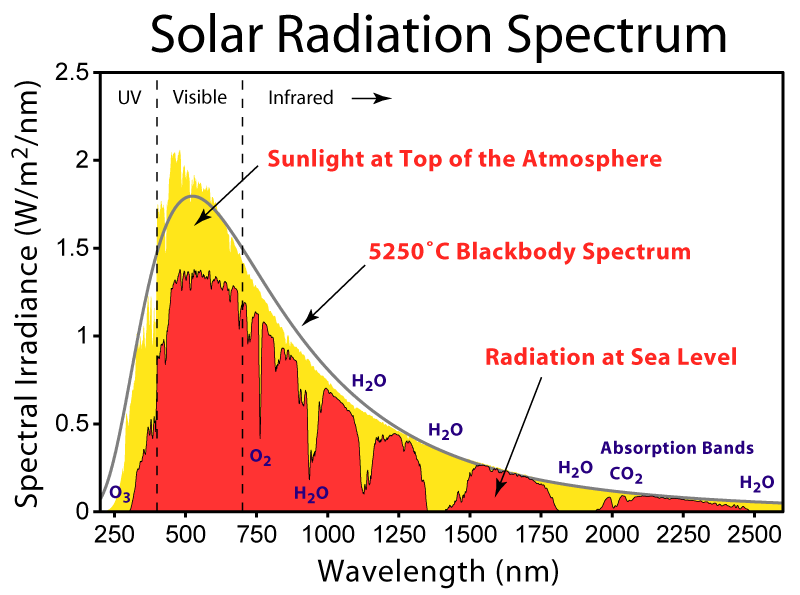
\includegraphics[width=100mm]{img/Solar_Spectrum.png}
\caption[Sonnenspektrum]{Der Vergleich von Spektrum des Sonnenlichtes im Weltall (AM0), der Strahlung eines schwarzen Körpers von 5250$^{\circ}$C und dem AM1.5 Spektrum. Quelle: \cite{sun}}\label{sunspec}
\end{figure}


\section{Sonnensimulator Aufbau}\thispagestyle{empty}


Mit der SolarConstant 4000 (siehe Abbildung \ref{sunsim}) der Firma Atlas kann die Einwirkung der Sonne auf Testobjekte simuliert werden. Dazu ist das Gerät mit zehn Metallhalogenid-Strahlungsquelle Lampen zu je 4kW. Durch die Füllung der Lampen mit Halogeniden wird ein kontinuierliches Spektrum erzeugt. Die Leuchten mit Filterscheiben ausgestattet, die das abgestrahlte Licht möglichst dem AM1.5 Spektrum ähnlich macht.
Jede Lampe wird von einem eigenen elektronisch geregelten Vorschaltgerät versorgt, welches für einen gleichmäßigen und flimmerfreien Betrieb sorgt.
Da die Lampen nicht für eine Heißzündung ausgelegt sind, und dabei eventuell zerstört werden können, ist eine Sperrzeit von 10 Minuten zum Abkülen vorgesehen, bevor die Lampen wieder eingeschaltet werden können.
Die Strahlungsleistung lässt sich reduzieren indem das gesamte Lampenfeld in die Höhe gefahren wird.
Weiters lässt sich die Bestrahlungsstärke einzelner Lampen über die Variation der elektrischen Leistung des Vorschaltgerätes varieren.
Allerdings führt eine Variation der elektrischen Leistung zu einer Änderung der spektralen Strahlungsverteilung. Es wir dvom Hersteller empfohlen, die Helligkeit der Lampen nur zwischen 80 und 100 \% zu variieren.
Die Testobjekte werden mittels Prüfgut-Einschub in einem Windkanal positioniert, dessen obere Abdeckung aus einem geeigneten Solarglas besteht. Die geneigte Glasplatte bewirkt eine Querschnittreduktion des Luftkanales und somit eine Erhöhung der Strömungsgeschwindigkeit zwischen Zuluft- und Abluftseite. Diese stetige Erhöhung der Geschwindigkit ist notwendig, damit die sich erwärmende Zuluft eine konstante Kühlwirkung hat, um die Testobjekt auf konstanter Temperatur zu halten.


\begin{figure}[htbp]
\centering
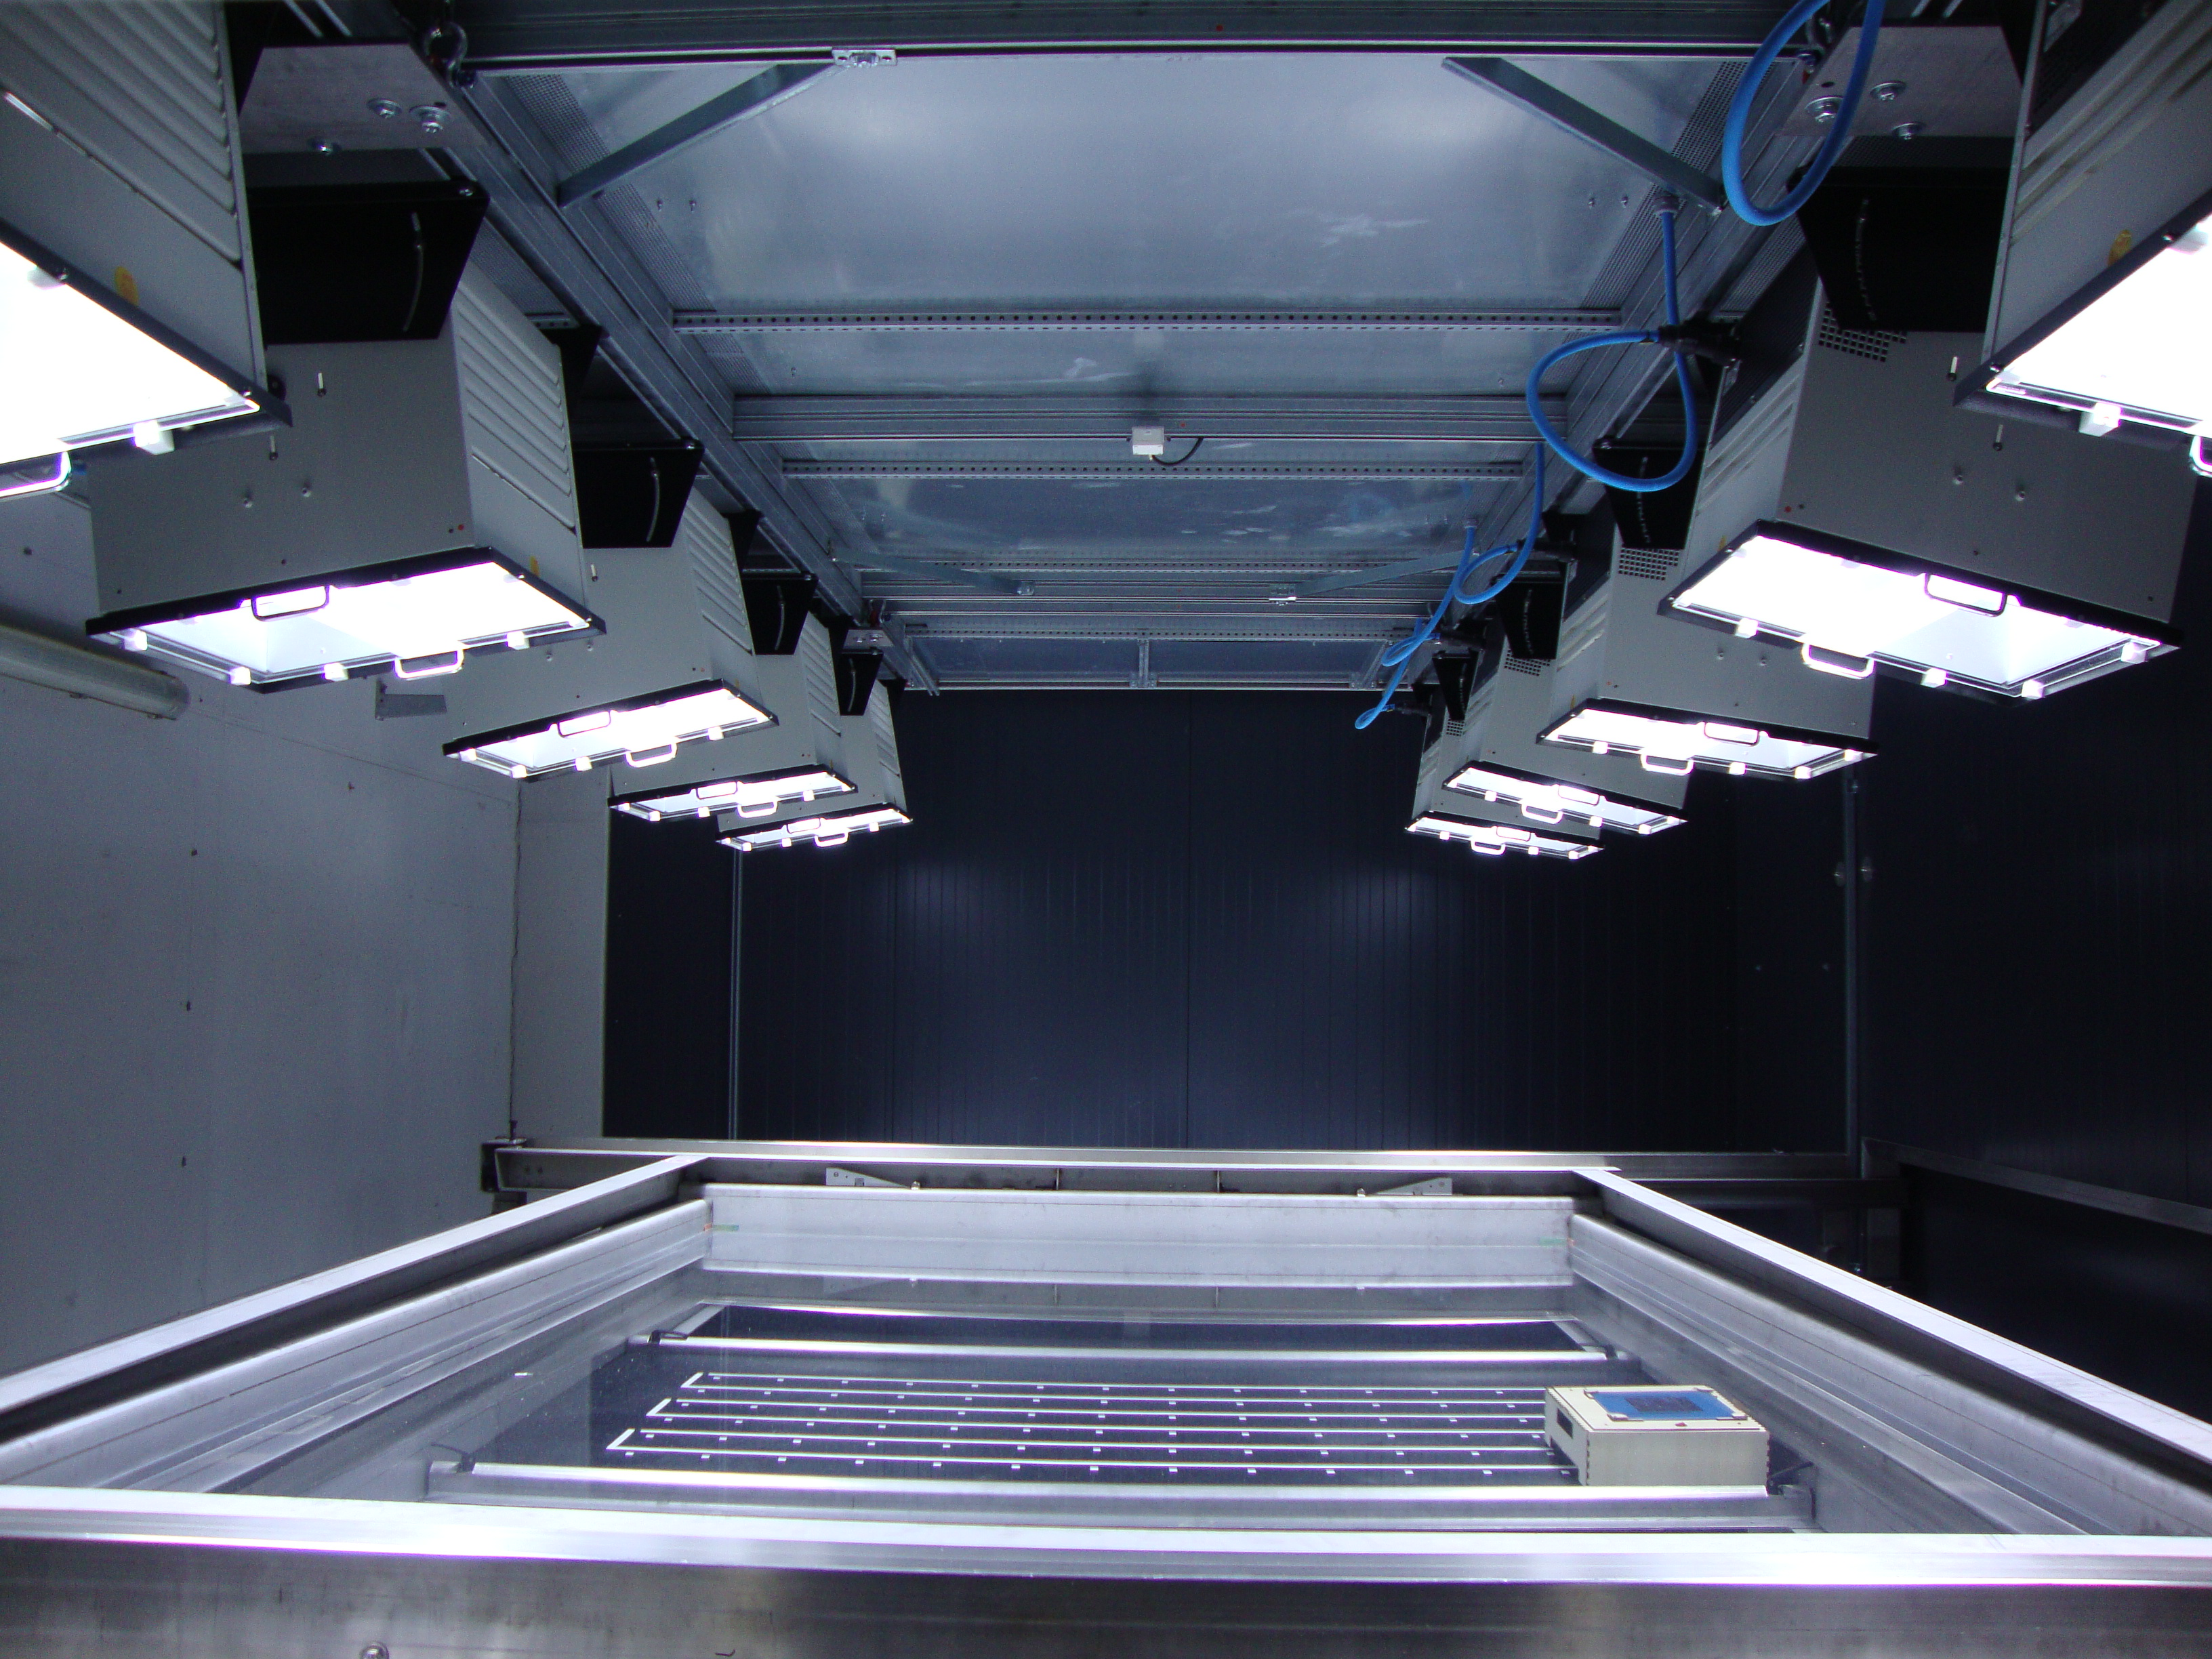
\includegraphics[width=100mm]{img/sunsimulator.jpg}
\caption[Sonnensimulator]{Der Aufbau des Sonnensimulators: Die 10 Metallhalogenoid Strahler, der Windkanal und die Prüfebene sind zu erkennen}\label{sunsim}
\end{figure}


\section{Anforderungen}\thispagestyle{empty}
Die Norm IEC 60904-9 \cite{norm9} stellt Anforderungen an Sonnensimulatoren. Ein Sonnensimulator wird anhand von 3 Kriterien bewertet: 
\begin{itemize}
\item die spektrale Übereinstimmung mit dem in Tabelle \ref{TabS1} aufgelisteten Wellenlängenbereichen. Zum AM1.5 Referenzspektrum sind durch die großen Schranken erhebliche Unterschiede möglich.
\begin{table}[htbp]
\centering
\begin{tabular}{ | c | c | c |}\hline
{\bf } & {\bf Wellenlängenbereich in nm} & {\bf \% der totalen Einstrahlung}\\ \hline
\hline
1  & 400 - 500 & 18,4 \\ \hline
2  & 500 - 600 & 19,9\\ \hline
3  & 600 - 700 & 18,4\\ \hline
4  & 700 - 800 & 14,9\\ \hline
5  & 900 - 900 & 12,5\\ \hline
6  & 900 - 1100 & 15,9\\ \hline
\end{tabular}
\caption{Spektralle Strahlungsverteilung nach IEC 60904-9}\label{TabS1}
\end{table}
\item die Gleichmäßigkeit der Bestrahlungsstärkeverteilung über die Testfläche
	\begin{equation}
 Non-uniformity (\%) = [\frac{max irradiance - min irradiance}{max irradiance + min irradiance}] \times (100%)
\end{equation}
\item die zeitliche Stabilität der Einstrahlung.
\begin{equation}
 Temporal (\%) = [\frac{max irradiance - min irradiance}{max irradiance + min irradiance}] \times (100%)
\end{equation}
\end{itemize}



Tabelle \ref{TabS2} gibt die Anforderungen an, nach denen Sonnensimulatoren in den Klassen A,b und C klassifiziert werden. Die Sonnensimulatorklasse ABB bedeutet eine 0,75- bis 1,25-fache Übereinstimmung in allen in Tabelle \ref{TabS1} angeführten Schranken, eine Homogenität der Einstrahlung zwischen 2\% und 5\% im Messbereich, und eine zeitliche Stabilität zwischen 2\% und 5\%. 
\begin{table}[htbp]
\centering
\begin{tabular}{ | c | c | c | c | c |}\hline
\multirow{2}{*}{Klassifikation} &  Spektrale  &  Örtliche  & {Kurzzeit-}& {Langzeit-}\\
& Übereinstimmung & Homogenität & {stabilität} & {stabilität} \\ 
\hline
\hline
A  & 0,75 - 1,25 & 2 \% & 0,5 \% & 2 \%\\ \hline
B  & 0,6 - 1,4 & 5 \% & 2 \% & 5 \%\\ \hline
C  & 0,4 - 2,0 & 10 \% & 10 \% & 10 \%\\ \hline

\end{tabular}
\caption{Anforderungen an die 3 verschiedenen Simulatorklassen}\label{TabS2}
\end{table}



\section{Theorie Referenzzelle}\thispagestyle{empty}
Es gibt verschiedene Solarzelltechnologien. Wirtschaftlich bedeutend sind im Moment nur kristalline Siliziumzellen und Dünnschichtzellen. Die kristallinen Siliziumzellen werden in monokristalline Zellen und multikristalline Zellen unterschieden. Beide zusammen machen über 80\% des weltweiten Photovoltaikmarktes aus \cite{iea00}. Als Referenzzelle für Messungen werden ausschließlich kristalline Zellen verwendet. Eine Referenzzellen ist eine genau vermessene Solarzellen, die als Strahlungsmessgerät dient. Wichtig ist, dass die Referenzzelle eine ähnliche spektralle Empfindlichkeit hat wie die zu messenden Zelle bzw. das zu messende Modul.
Siliziumsolarzellen bestehen aus einer großflächigen Diode. Die Sperrschicht ist dabei dem Sonnenlicht ausgesetzt. Gelangt ein Lichtquanten in die Sperrschicht kann aufgrund des inneren Photoeffektes ein Elektron/Loch Paar erzeugt werden. Durch das elektrische Feld in der Sperrschicht werden die Ladungsträger getrennt bevor sie kombinieren können. Elektronen bewegen aufgrund ihrer negativen Ladung entgegen der Feldrichtung in die n-Zone. Löcher wandern in Feldrichtung zur Raumladungsfreien p-Zone. Die Leerlaufspannung einer Solarzelle ist kleiner als die Diffusionsspannung, der Spannung über die Raumladungszone, die der Diffusion von Ladungsträgern entgegenwirkt.
\begin{figure}[htbp]
\centering
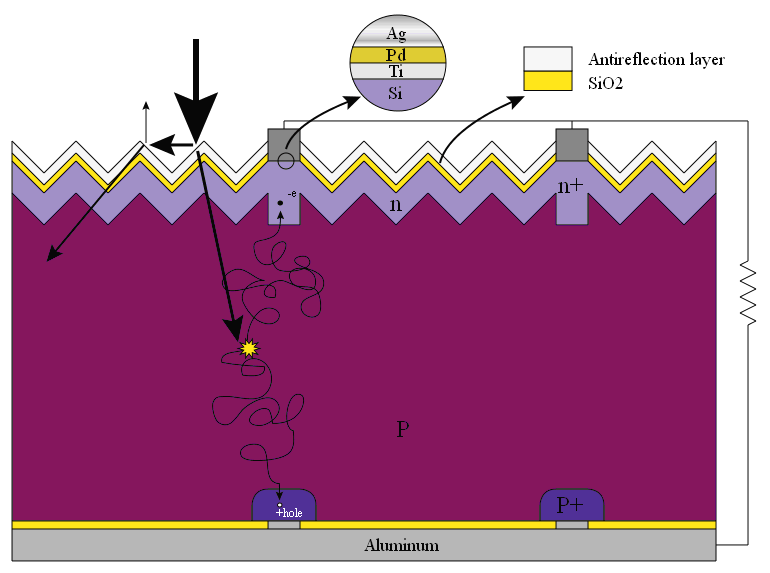
\includegraphics[width=125mm]{img/cell.png}
\caption{Der Schematischer Aufbau einer Siliziumsolarzelle. Quelle: \cite{cell}}\label{cell}
\end{figure}


Die unbeleuchtete Solarzelle ist funktioniert wie eine normale Halbleiterdiode, die einen Durchlassstrom von p- nach n-Seite fließen lässt, falls eine Spannung von p nach n anliegt. Bei Beleuchtung wird zusätzlich ein Photostrom erzeugt, welcher proportional zur Bestrahlungsstärke und der Zellfläche ist. Das Eindiodenmodel (siehe Abbildung ~\ref{esb}) besteht daher aus einer Stromquelle, dazu parallel einer Diode, einen Parallelwiderstand und einem Serienwiderstand. Der Parallelwiderstand fasst Kurzschlüsse zusammen, die realen Solarzellen am Rand oder an den Korngrenzen auftreten können. Mit dem Serienwiderstand werden alle Spannungsabfälle in der Solarzelle erfasst. Eine ideale Solarzelle hat einen Serienwiderstand von null und einen Parallelwiderstand von unendlich. 
\begin{figure}[htbp]
\centering
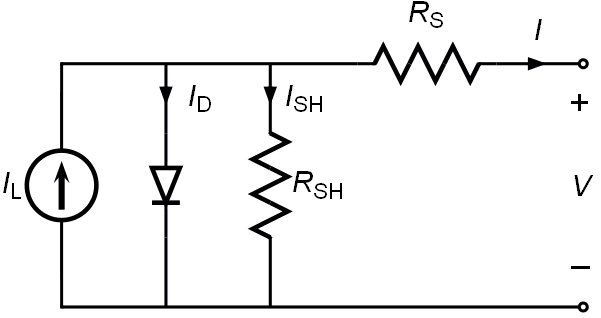
\includegraphics[width=100mm]{img/esb.png}
\caption{Das Eindiodenmodell einer Sorlarzelle. Quelle: \cite{esb}}\label{esb}
\end{figure}

Durch den zusätzlichen Photostrom verschiebt (siehe Abbildung ~\ref{kennlinie}) sich die Diodenkennline. Im Leerlauf  bzw. Kurzschlussbetrieb gibt die Solarzelle keine Leistung ab. Der Punkt der Kennlinie mit der maximalen Leistung wird als Maximum Power Point (MPP) bezeichnet.

Der Füllfaktor berechnet sich aus Strom im maximalen Leistungspunkt $I_{mp}$, Spannung im maximalen Leistungspunkt $U_{mp}$, Kurzschlusstrom $I_{sc}$ und Leerlaufspannung $U_{oc}$ zu:
  \begin{equation}
     FF = \frac {I_{mp} U_{mp}} {I_{sc} U_{oc}}
  \end{equation}
Der Füllfaktor ist das Verhältnis der Fläche des Rechteckes mit den Seitenlängen I$_{mp}$ und U$_{mp}$ zu der Fläche des Rechteckes mit den Seitenlängen I$_{sc}$ und U$_{oc}$ (siehe Abbildung \ref{kennlinie}).

\begin{figure}[htbp]
\centering
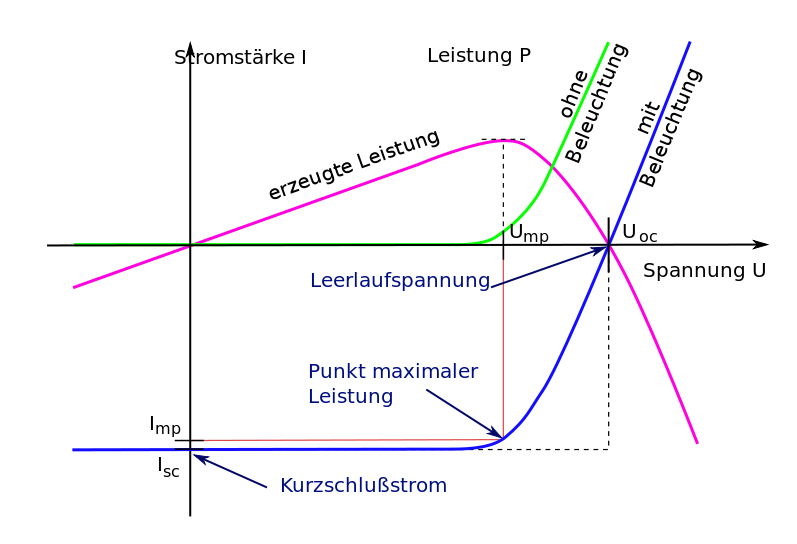
\includegraphics[width=125mm]{img/kennlinie.png}
\caption{Dunkel- und Hellkennlinien}\label{kennlinie}
\end{figure}

Die Kennlinie der Solarzelle ist von der Einstrahlung abhängig (siehe Abbildung \ref{mpp}). Der Kurzschlusstrom ist direkt proportional zur Einstrahlung.
Laut IEC 60891 [\cite{norm891}] berechnet sich die Einstrahlung aus dem gemessenen Kurzschlussstrom, den STC-Kurzschlussstrom, einen relativen Temperaturkoeffizienten und der Zelltemperatur:
\begin{equation}
G = \frac{1000Wm^{-2}I_{RC}}{I_{RC,STC}} [1 - \alpha_{RC}(T_{RC}-25^{\circ} C]
\end{equation}
\begin{figure}[htbp]
\centering
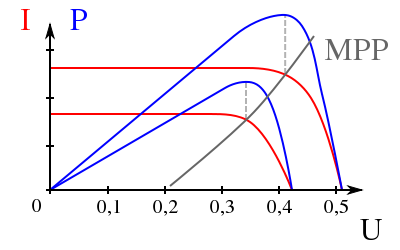
\includegraphics[width=75mm]{img/mpp.png}
\caption{Abhängigkeit des MPP von der Einstrahlung}\label{mpp}
\end{figure}

\chapter{Entwicklungsprozess}\thispagestyle{empty}

Diese Kapitel beschreibt die Entwicklung des Roboters und ist in 3 Unterabschnitte gegliedert: das mechanische Design, die Elektronik und die dazugehörige Software.
Einige Designelemente waren zu Beginn der Entwicklung vorgegeben. Der Roboter sollte mit Mecanum-Rädern ausgestattet sein. Er sollte eine photovoltaische Messzelle aufnehmen können. Er muss sich im Raum orientieren können. Die Materialien sollten UV beständig sein, da der Roboter in einer Umgebung mit starker UV arbeitet.
Die Mecanum-Räder erlauben es dem Roboter sich auch seitwärts fortzubewegen, die Längsachse des Roboters, und somit auch die Messzelle, während des gesamten Messvorganges die Orientierung im Raum beibehält. 

\section{Hardwaredesign und Komponenten}\thispagestyle{empty}

Dieser Abschnitt behandelt die Entwicklung der mechanischen Komponenten, diese sind die 4 Räder und die Chassis des Roboters. Die mögliche Bauhöhe ist durch den Windkanal im Sonnensimulator beschränkt, zusätzlich soll die Messzelle möglichst in der gleichen Höhe wie zu messende Module liegen.
Die Größe der Messzelle, zusammen mit dem Raddurchmesser und der Breite der Räder gibt eine Minimalabmessung vor die der Roboter nicht unterschreiten kann. Zusätzlich müssen noch die Motoren, der Akku und die Elektronik im Inneren des Roboters Platz finden.
Designprozess:
\begin{itemize}
\item Mecanumräder sind festgelegt
\item  Platz für Messzelle, oben, darunter Elektronik und Motoren
\item  Mecanum Räder innerhalb des Chassis, die Zelle befindet sich  am Dach
\item  Optische Sensoren zum Verfolgen einer Linie, da auch seitwärts gefahren werden soll, in der Mitte des Roboters an der Unterseite.
\item  Platz für den Mikrocontroller, die Elektronik, den Akku im Inneren. 
\item  Da wichtige Komponenten wie der Akku später gewechselt wurden, war es gut Reserveplatz zu haben.\end{itemize}

Der Roboter ist ein wenig zu groß geworden, die verwendete Messzelle ist kleiner als in den Planungen, dafür ist der Akku größer als ursprünglich gedacht. 

\subsection{Mecanum-Plattform}\thispagestyle{empty}
Mecanum-Räder erlauben einem Fahrzeug, ohne mechanischer Lenkung, sich in jede Richtung zu bewegen. Benannt ist es nach dem schwedischen Unternehmen Macanum, welches dieses Rad 1971 entwickelt hat.
Jedes Rad wird über einen eigenen Motor angetrieben, und verfügt über eine separate Ansteuerung. Die Räder bestehen aus einer Felge (siehe Abbbildung \ref{rad}), auf der unter einem Winkel von 45 Grad befestigte, ballige Rollen so angebracht sind, die über den Abrollumfang einen exakten Kreis bilden (siehe Abbbildung \ref{rad2}).

Durch die Schräganordnung der Laufrollen entstehen beim Antreiben eines Rades 2 Kraftkomponenten, eine in der Achse  und eine 90$^\circ$. Gegeneinander gerichtete Kräfte der einzelnen Räder werden über die Achsen und den Rahmen kompensiert. Die übrigen Kräfte addieren sich zur resultierenden Fahrtrichtung. Auf diese Weise sind durch entsprechendes Ansteuern der einzelnen Räder omnidirektionale Fahrmanöver möglich (siehe Abbildung \ref{fahrman}).

\begin{figure}
    \subfigure[Vor/Zurück]{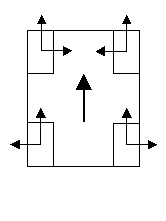
\includegraphics[width=50mm]{img/gerade.png}}
    \subfigure[Links/Rechts]{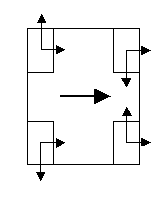
\includegraphics[width=50mm]{img/seitw.png}}
     \subfigure[Drehen]{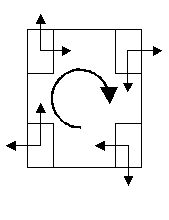
\includegraphics[width=50mm]{img/dreh.png}}
\caption{Einige mögliche Fahrmanöver eines Mecanum-Rad-Roboters}\label{fahrman}
\end{figure} 

\begin{figure}[htbp]
\centering
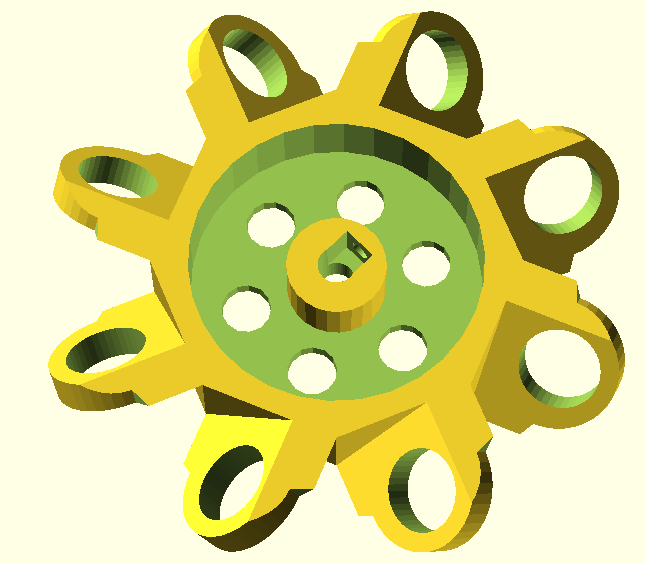
\includegraphics[width=75mm]{img/wheel.png}
\caption{Die Felge des Mecanum Rades}\label{rad}
\end{figure}

\begin{figure}[htbp]
\centering
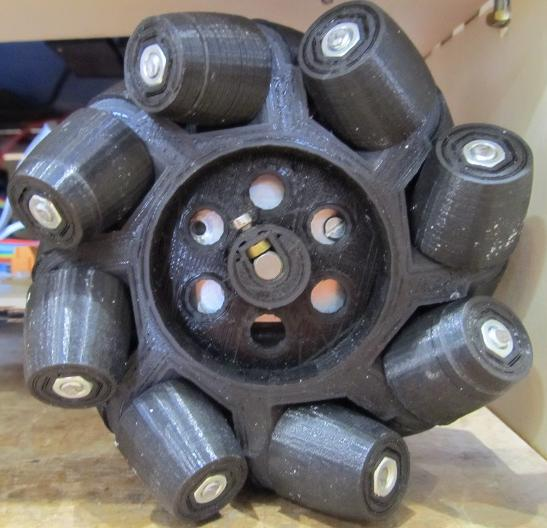
\includegraphics[width=75mm]{img/rad.jpg}
\caption{Ein fertig Rad, montiert am Roboter.}\label{rad2}
\end{figure}

Jedes der vier Räder besteht aus einer Felge, insgesamt 16 Laufrollen, 8 Kugellager, 8 M4x45mm Schraube, 8 M4 Muttern, sowie 16 M4 Beilagscheiben. 
Das Rad ist mit einer M3 Schraube und einer M3 Mutter an der Motorachse fixiert.
Die Felgen und die Laufrollen wurden mit einem 3D-Drucker gefertigt. 
Die Vorlage namens Mecanum Wheel MK2 stammt von http://www.thingiverse.com/thing:2473, und kann unter der Attribution-NonCommercial-ShareAlike 3.0 Unported Lizenz nicht kommerziell verwendet werden.
Die Laufrollen so angepasst, dass die Mutter bzw. der Schraubenkopf in der Rolle versenkt ist, damit das Rad insgesamt kompakter ist. Zum bearbeiten wurde OpenSCAD, ein 3D-Compiler, verwendet. 
Die Kugellager wurden in die Falgen eingeklebt,
\newline
\newline
Ab hier Entwurf: Mehr aud SCAD eingehen? Druckvorbereitung. Genauer den Druck beschreiben? Multidruck der Rollen. 
Probedrücke bis endgültige Rolle gefunden wurde.
Druckzeit: Felge rund drei Stunden, eine Rolle etwa 20 Minuten.
3D-Drucker war fehleranfällig. Wartungintensiv. Druckmaterial: AMS-Kunststoff (Datenblatt wäre nett!)

Analyse von einem ABS-Kunststoff: Characterization of Material Properties
$http://www.stratasys.com/sitecore/shell/Applications/~/media/Fortus/Files/PDFs/MaterialPropertiesReport-ABS-M30.pdf?utm_source=materials_study_news_release_August_2011$ 

Temperatur hat Einfluss auf Materialeigenschaften, es ist gut, dass der Kunststoff vor direkter Sonneneinstrahlung, und somit Erwärmung geschützt ist, besonders da er schwarz ist.
ABS ist grundsätzlich UV beständig, findet z.B. Anwendung in Rasenmähern. "If UV-stabilizators are added, ABS is suitable for outdoor applications." 
Genauer Typ von ABS unbekannt. 
Zwei verschiedene Radtypen, Rollen gleich, unterschiedliche Felgen. Anordnung siehe Bild. Montage so, dass die Räder symmetrisch sind. Symmetrische Anordnung der Räder.
Das Material für den 3D-Druck ist ABS (Acrylnitril-Butadien-Styrol). Es besitzt eine hohe Oberflächenhärte (ist damit für kratzfeste und matt glänzende Oberflächen geeignet), besitzt eine gute Schlagfestigkeit. Es schmilzt in einem Temperaturbereich von 220 - 250 $^\circ$C (Hochtemperatur-ABS-Blends noch höher) und kann im flüssigen Zustand im Spritzgussverfahren oder per Extruder geformt werden. Als eine spezielle Form letzterer Methode stellt das Material auch üblicherweise den Werkstoff dar, der von 3D-Druckern verdruckt wird. Standard-ABS erweichen um 95 - 110 $^\circ$C (siehe Vicat-Erweichungstemperatur). 
Nachteil beim 3D-Druck ist die Beschränkung auf einen Werkstoff. 


\subsection{Chassis}\thispagestyle{empty}

\noindent Das Chassis wurde aus Sperrholz gefertigt. Dieses Material wurde gewählt weil es leicht zu bearbeiten, robust und UV-beständig ist. Das Design wurde mit QCAD entwickelt. QCAD ist ein 2-dimensionales CAD Programm. 
Die Abmessungen des Chassis wurde im Wesentlichen abgestimmt auf: \begin{itemize}
\item Den Durchmesser und der Breite der Mecanum Räder, die innerhalb des Chasis liegen, damit die Räder vor der UV Strahlung geschützt sind, kein Einfluss (Beschattung oder Reflexionen) auf die Messzelle besteht.
\item Die Größe der Motoren.
\item Den Arduino-Mikrocontroller , die Motorsteuerelektronik und die Messelektronik
\item Den Akku zur Stromversorgung, die dazugehörende Akku Spannungsüberwachung 
\item Die Abmessung der eingekapselten Solarzelle.
 \end{itemize}

Das Chassis besteht aus der Bodenplatte, den Seitenwänden und der oberen Abdeckung mit der Aufnahme für die Messzelle (siehe Abbildung \ref{gehause}). Zur Verringerung des Luftwiderstandes sind zwei Seitenwände geneigt (siehe Abbildung \ref{robo3d}).  
\noindent Die Einzelteile wurden mit einem Lasercutter aus einer Sperrholzplatte geschnitten. Die Einzelteile wurden teilweise miteinander verleimt. Damit eine zukünftige Wartung problemlos möglich ist, wurde der Aufbau verschraubt ausgeführt.
Die Motoren sind verschraubt, damit ein Austausch möglich ist. Einzelne Räder als auch die Rollen lassen sich bei Bedarf austauschen. 
Das Chassis besteht aus der Bodenplatte, den Seitenwänden und der oberen Abdeckung mit der Aufnahme für die Messzelle (siehe Abbildung \ref{gehause}). Zur Verringerung des Luftwiderstandes sind zwei Seitenwände geneigt (siehe Abbildung \ref{robo3d}).  


\begin{figure}[htbp]
\centering
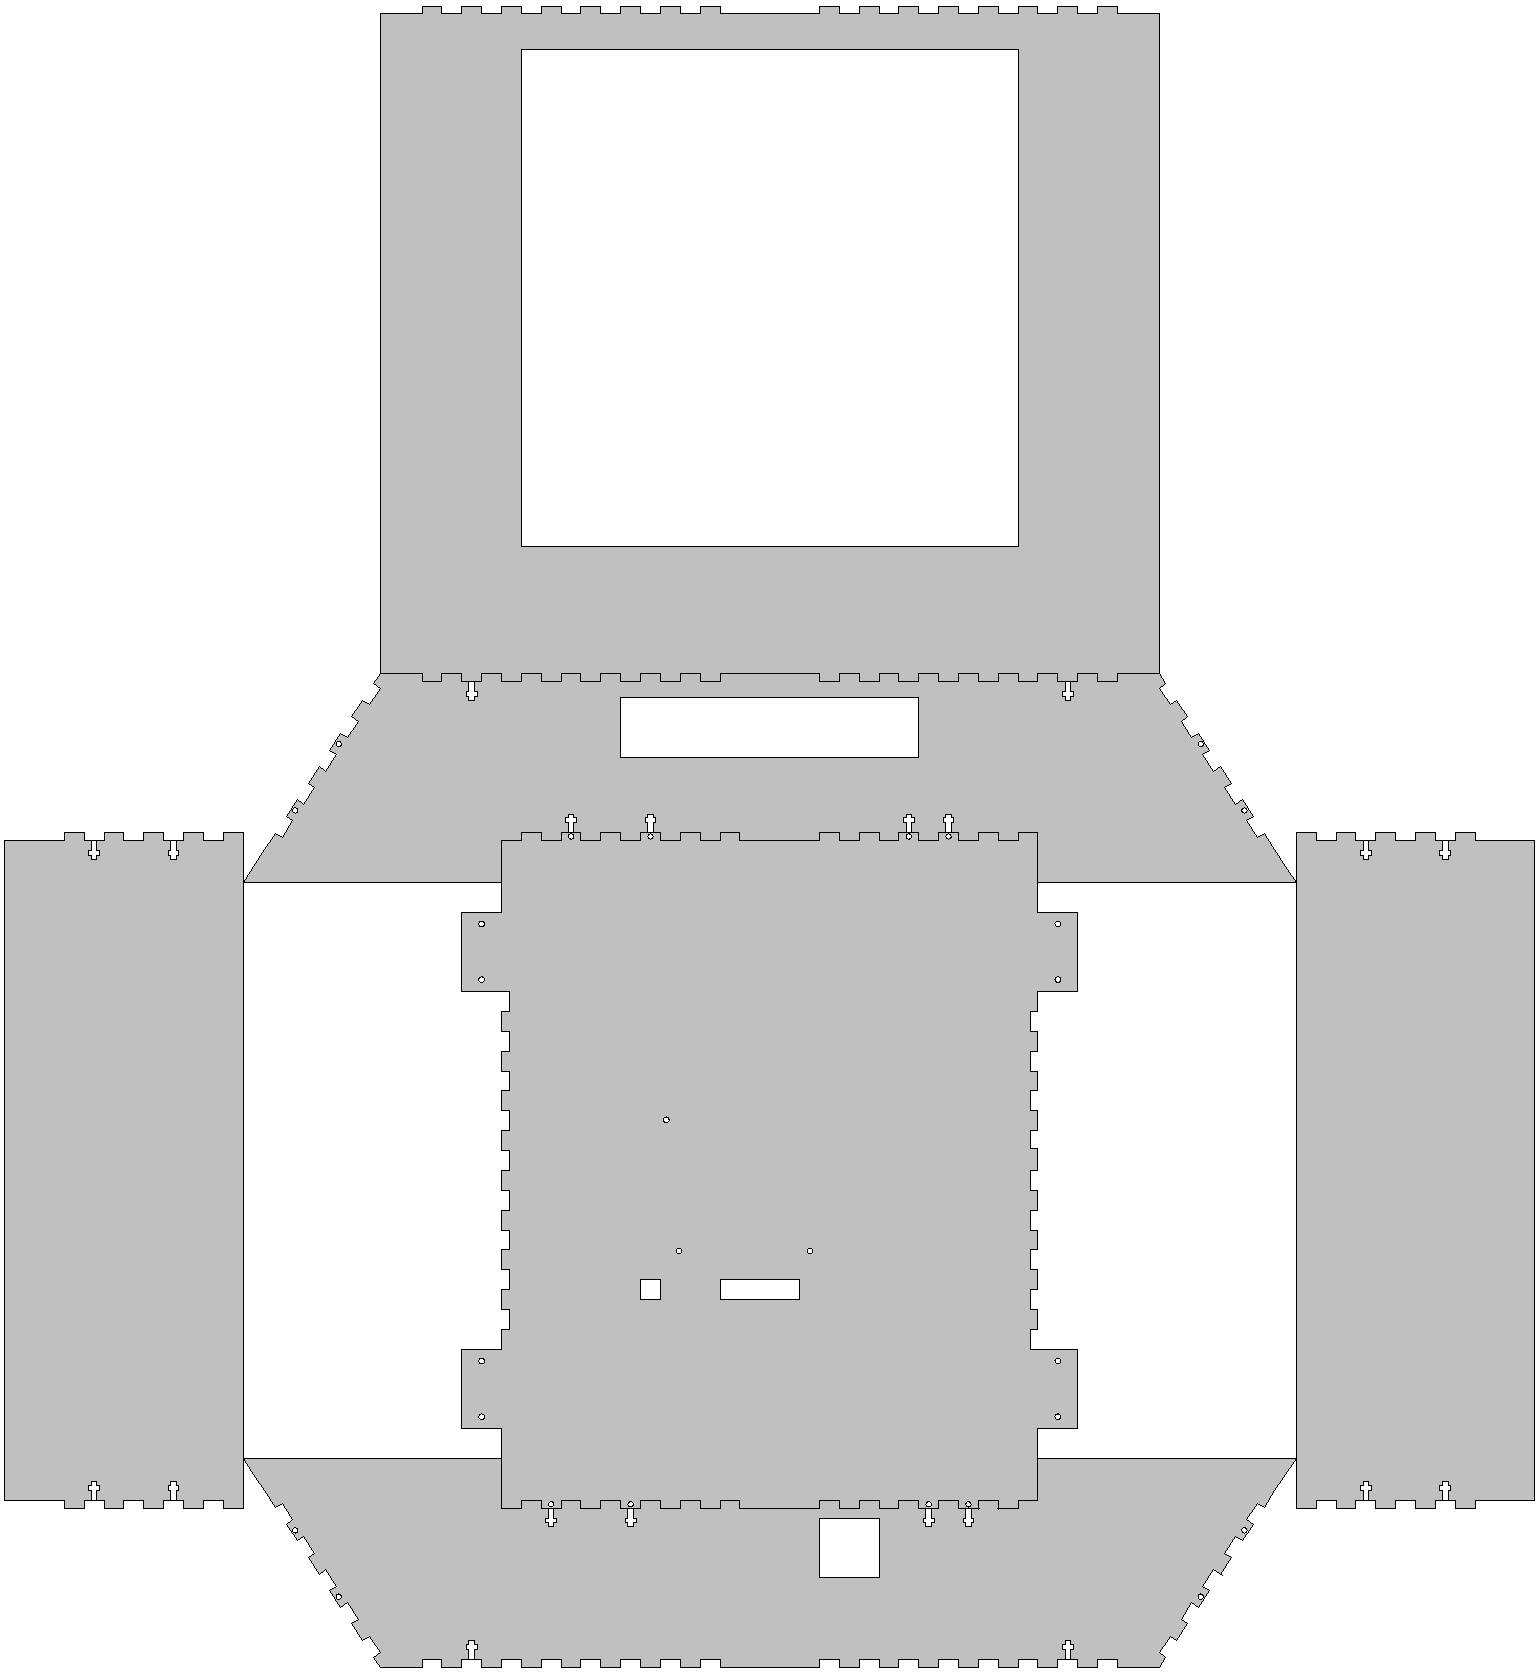
\includegraphics[width=125mm]{img/gehause3.png}
\caption[Chassis]{Die Schnittvorlage des Chassis}\label{gehause}
\end{figure}

\begin{figure}[htbp]
\centering
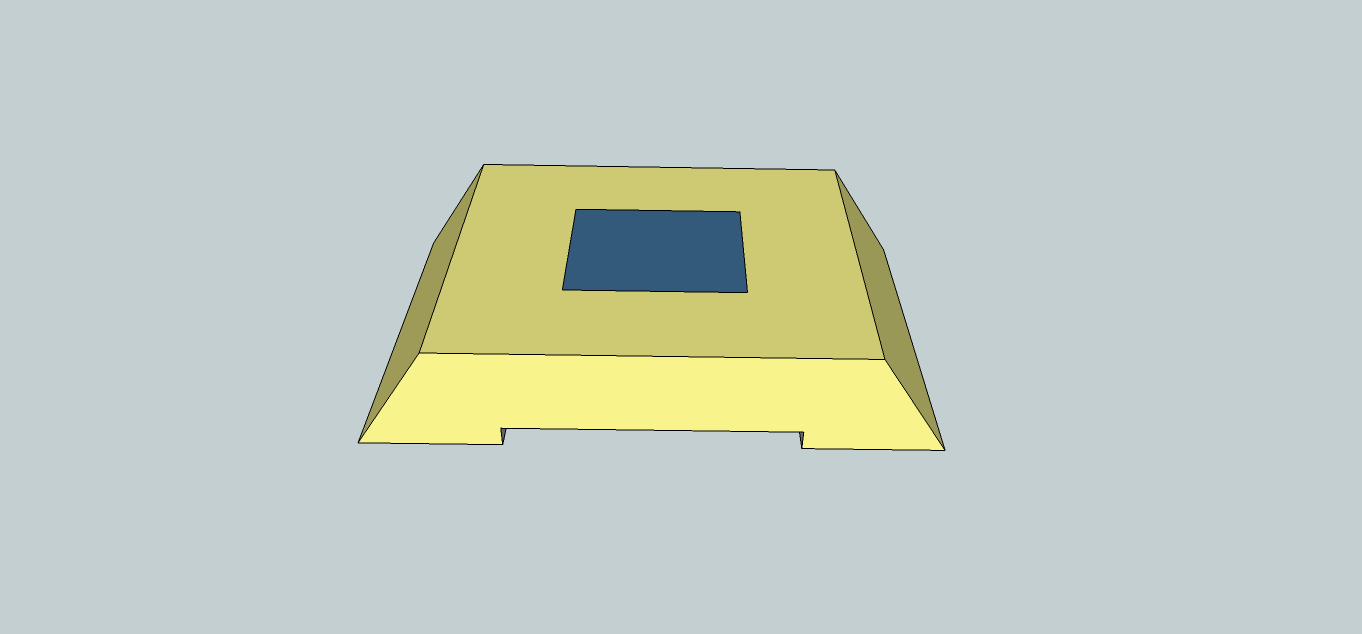
\includegraphics[width=125mm]{img/robo3d.png}
\caption[Chassis]{Ein 3D-Modell der Chassis}\label{robo3d}
\end{figure}


\section{Steuerungselektronik}\thispagestyle{empty}

Dieser Abschnitt beschreibt die Entwicklung der Elektronik. Die Funktionalität wurde auf verschiedene Module aufgeteilt. Das erleichtert die Platzierung der Elektronik innerhalb des Messroboters, und den Austausch von Komponenten im Fehlerfall. 
Das Gehirn des Roboters ist ein Arduino Mega 2560 Mikrocontroller Board. Darauf aufgesteckt ist ein sogenanntes Shield, eine selbst entwickelte Platine, das die $\pm$5V Spannungsversorgung, die Schnittstellen zu den anderen Platinen und einen SD-Karten Einschub beheimatet.
Es gibt 3 Messplatinen, eine für den Kurzschlussstrom der Messzelle, zwei für Temperaturmessungen. Eine Platine überwacht den Ladezustand des Akkus. Die Steuerung der vier Motoren ist auf einer Platine zusammengefasst.
Die einzelnen Komponenten sind wie in Abbildung \ref{elek} auf der Bodenplatte angeordnet.
\begin{figure}[htbp]
\centering
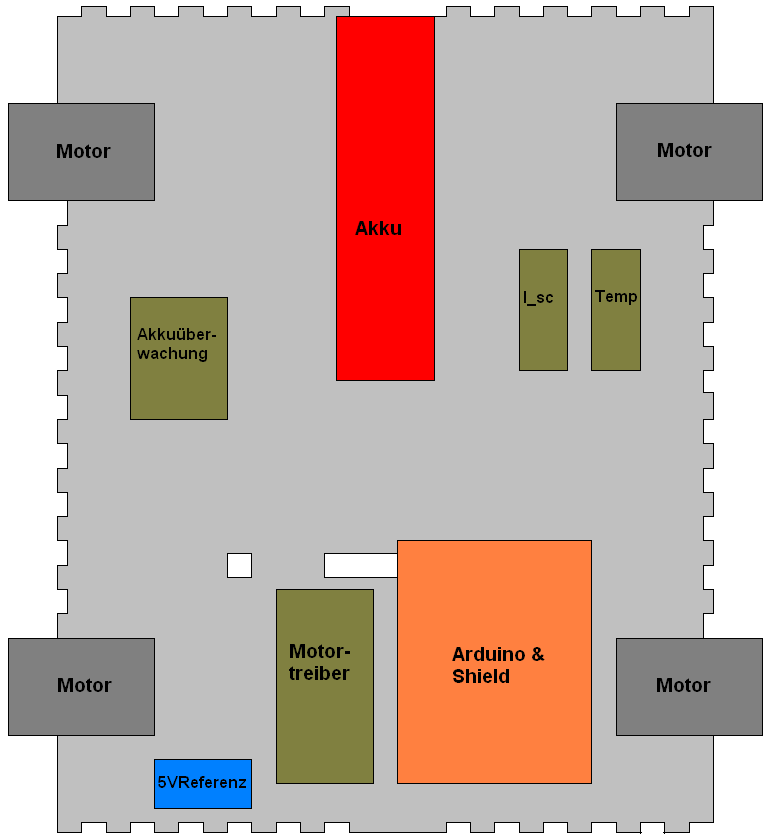
\includegraphics[width=100mm]{img/bodenplatte.png}
\caption{Die Anordnung der Elektronik auf der Bodenplatte im Roboter}\label{elek}
\end{figure}
 
\subsection{Motorensteuerung}\thispagestyle{empty}

Die Motorplatine \ref{hbridge2} besteht aus zwei integrierten H-Brücken-Bausteinen (IC1, IC2), einer 16 poligen Buchse und fünf zweipoligen Buchsen für die Stromversorgung und den Anschluss der vier Motoren. Bei den integrierten H-Brücken-Baustein handelt es sich um einen NJM2670 \cite{njm}, welcher zwei H-Brücken in einem Baustein vereint, zusätzlich verfügen diese Bausteine über eine interne Logik, welche Kurzschlüsse über die Brücke unmöglich macht.
Die Drehzahl der Motoren wird mit Pulsweitenmodulation variiert. Dabei ist es wichtig, dass die Transistoren in der Brücke schnell genug schalten können. Die PWM-Ausgänge des Arduino arbeiten mit einer Frequenz von etwa 500Hz \cite{pwm}.
Die Gleichspannungsmotoren sind Getriebemotoren mit der Bezeichnung RB 35, und einem Übersetzungsverhältnis von 1:200. Die maximale Versorgungsspannung wurde mit 12V angegeben. Die Leerlaufdrehzahl beträgt bei 12V Versorgungsspannung 20 Umdrehungen pro Minute.
Der Roboter wird mit einem Lithium-Ionen-Akku versorgt. Die Spannung beträgt, abhängig vom Ladezustand zwischen 16,4V und 15,0V. Damit es zu keiner Überlastung der 12V-Motoren, kommt wurde bei der Pulsweitenmodulation ein maximales Tastverhältnis von 50\% eingehalten.
 

\begin{figure}[htbp]
\centering
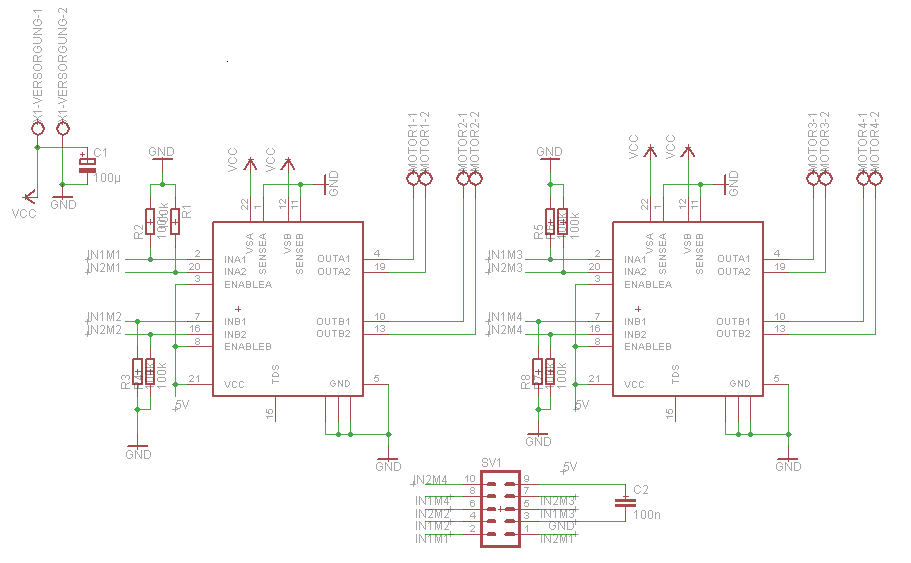
\includegraphics[width=150mm]{img/HBrucke.png}
\caption{Der Schaltplan der Motortreiberplatine.}\label{hbridge2}
\end{figure}


\subsection{Optische Sensorik}\thispagestyle{empty}
Der Roboter orientiert sich an einer aus geraden Teilstücken bestehenden Linienfolge. Die Linie ist weiß auf dunklem Untergrund.
Als Sensor wurde ein CNY70 verwendet. Der CNY 70 ist ein Reflexionsensor. Der Sensor wird in einem fixen Abstand zu einer Ebene montiert. Eine LED sendet Licht mit 950nm aus, welches an der Ebene reflektiert wird. Damit können Unterschiede des Reflektionkoeffizienten, umgangssprachlich der Farbe, gemessen werden. Die Anordung 9 solcher Sensoren in einem 3 mal 3 Array kann sowohl vertikale als auch horizontale Linien erkennen, sowie Ecken.

\begin{figure}[htbp]
\centering
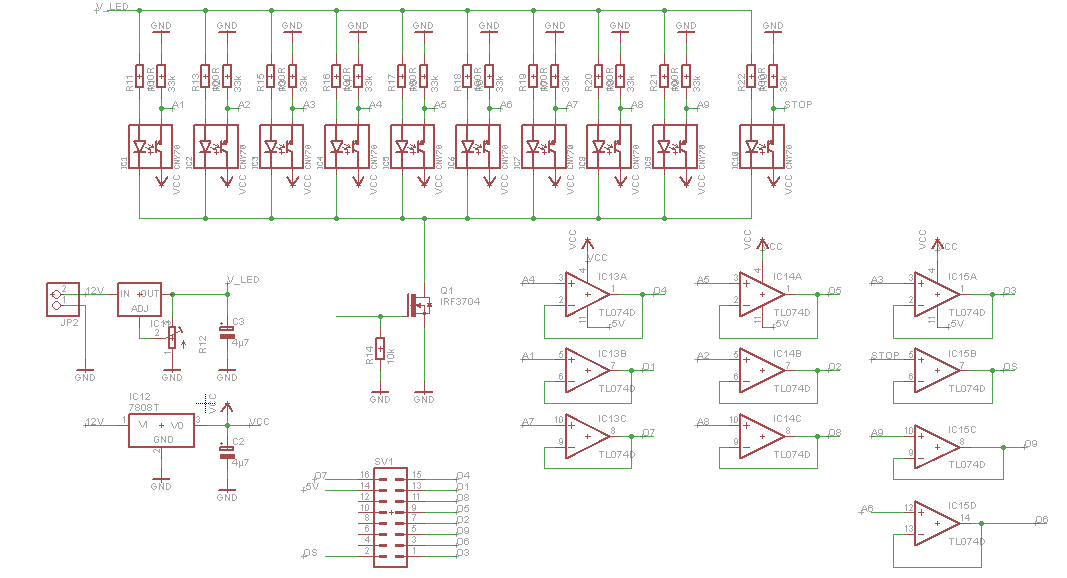
\includegraphics[width=125mm]{img/array.png}
\caption{Der Schaltplan des Sensorarrays}\label{array}
\end{figure}

\begin{figure}[htbp]
\centering
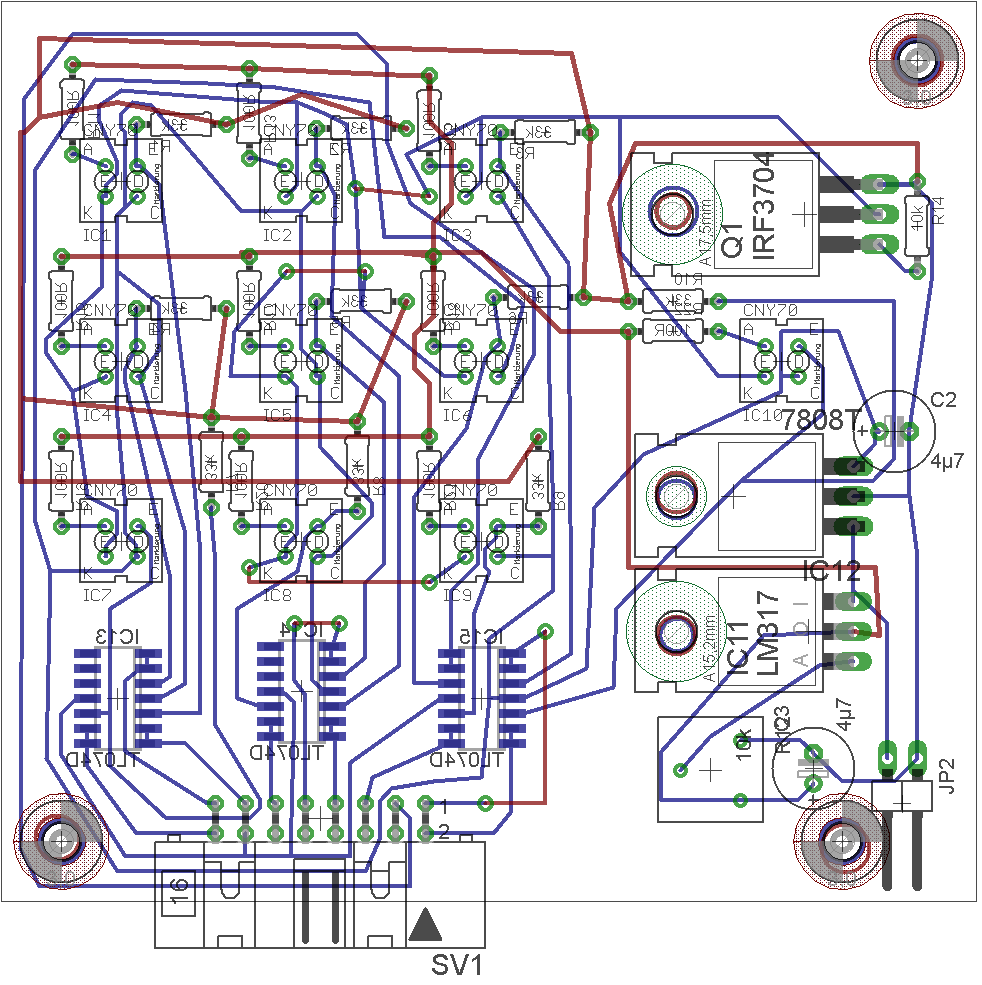
\includegraphics[width=125mm]{img/array21.png}
\caption{Das Layout des Senorarrays}\label{array2}
\end{figure}


\begin{figure}[htbp]
\centering
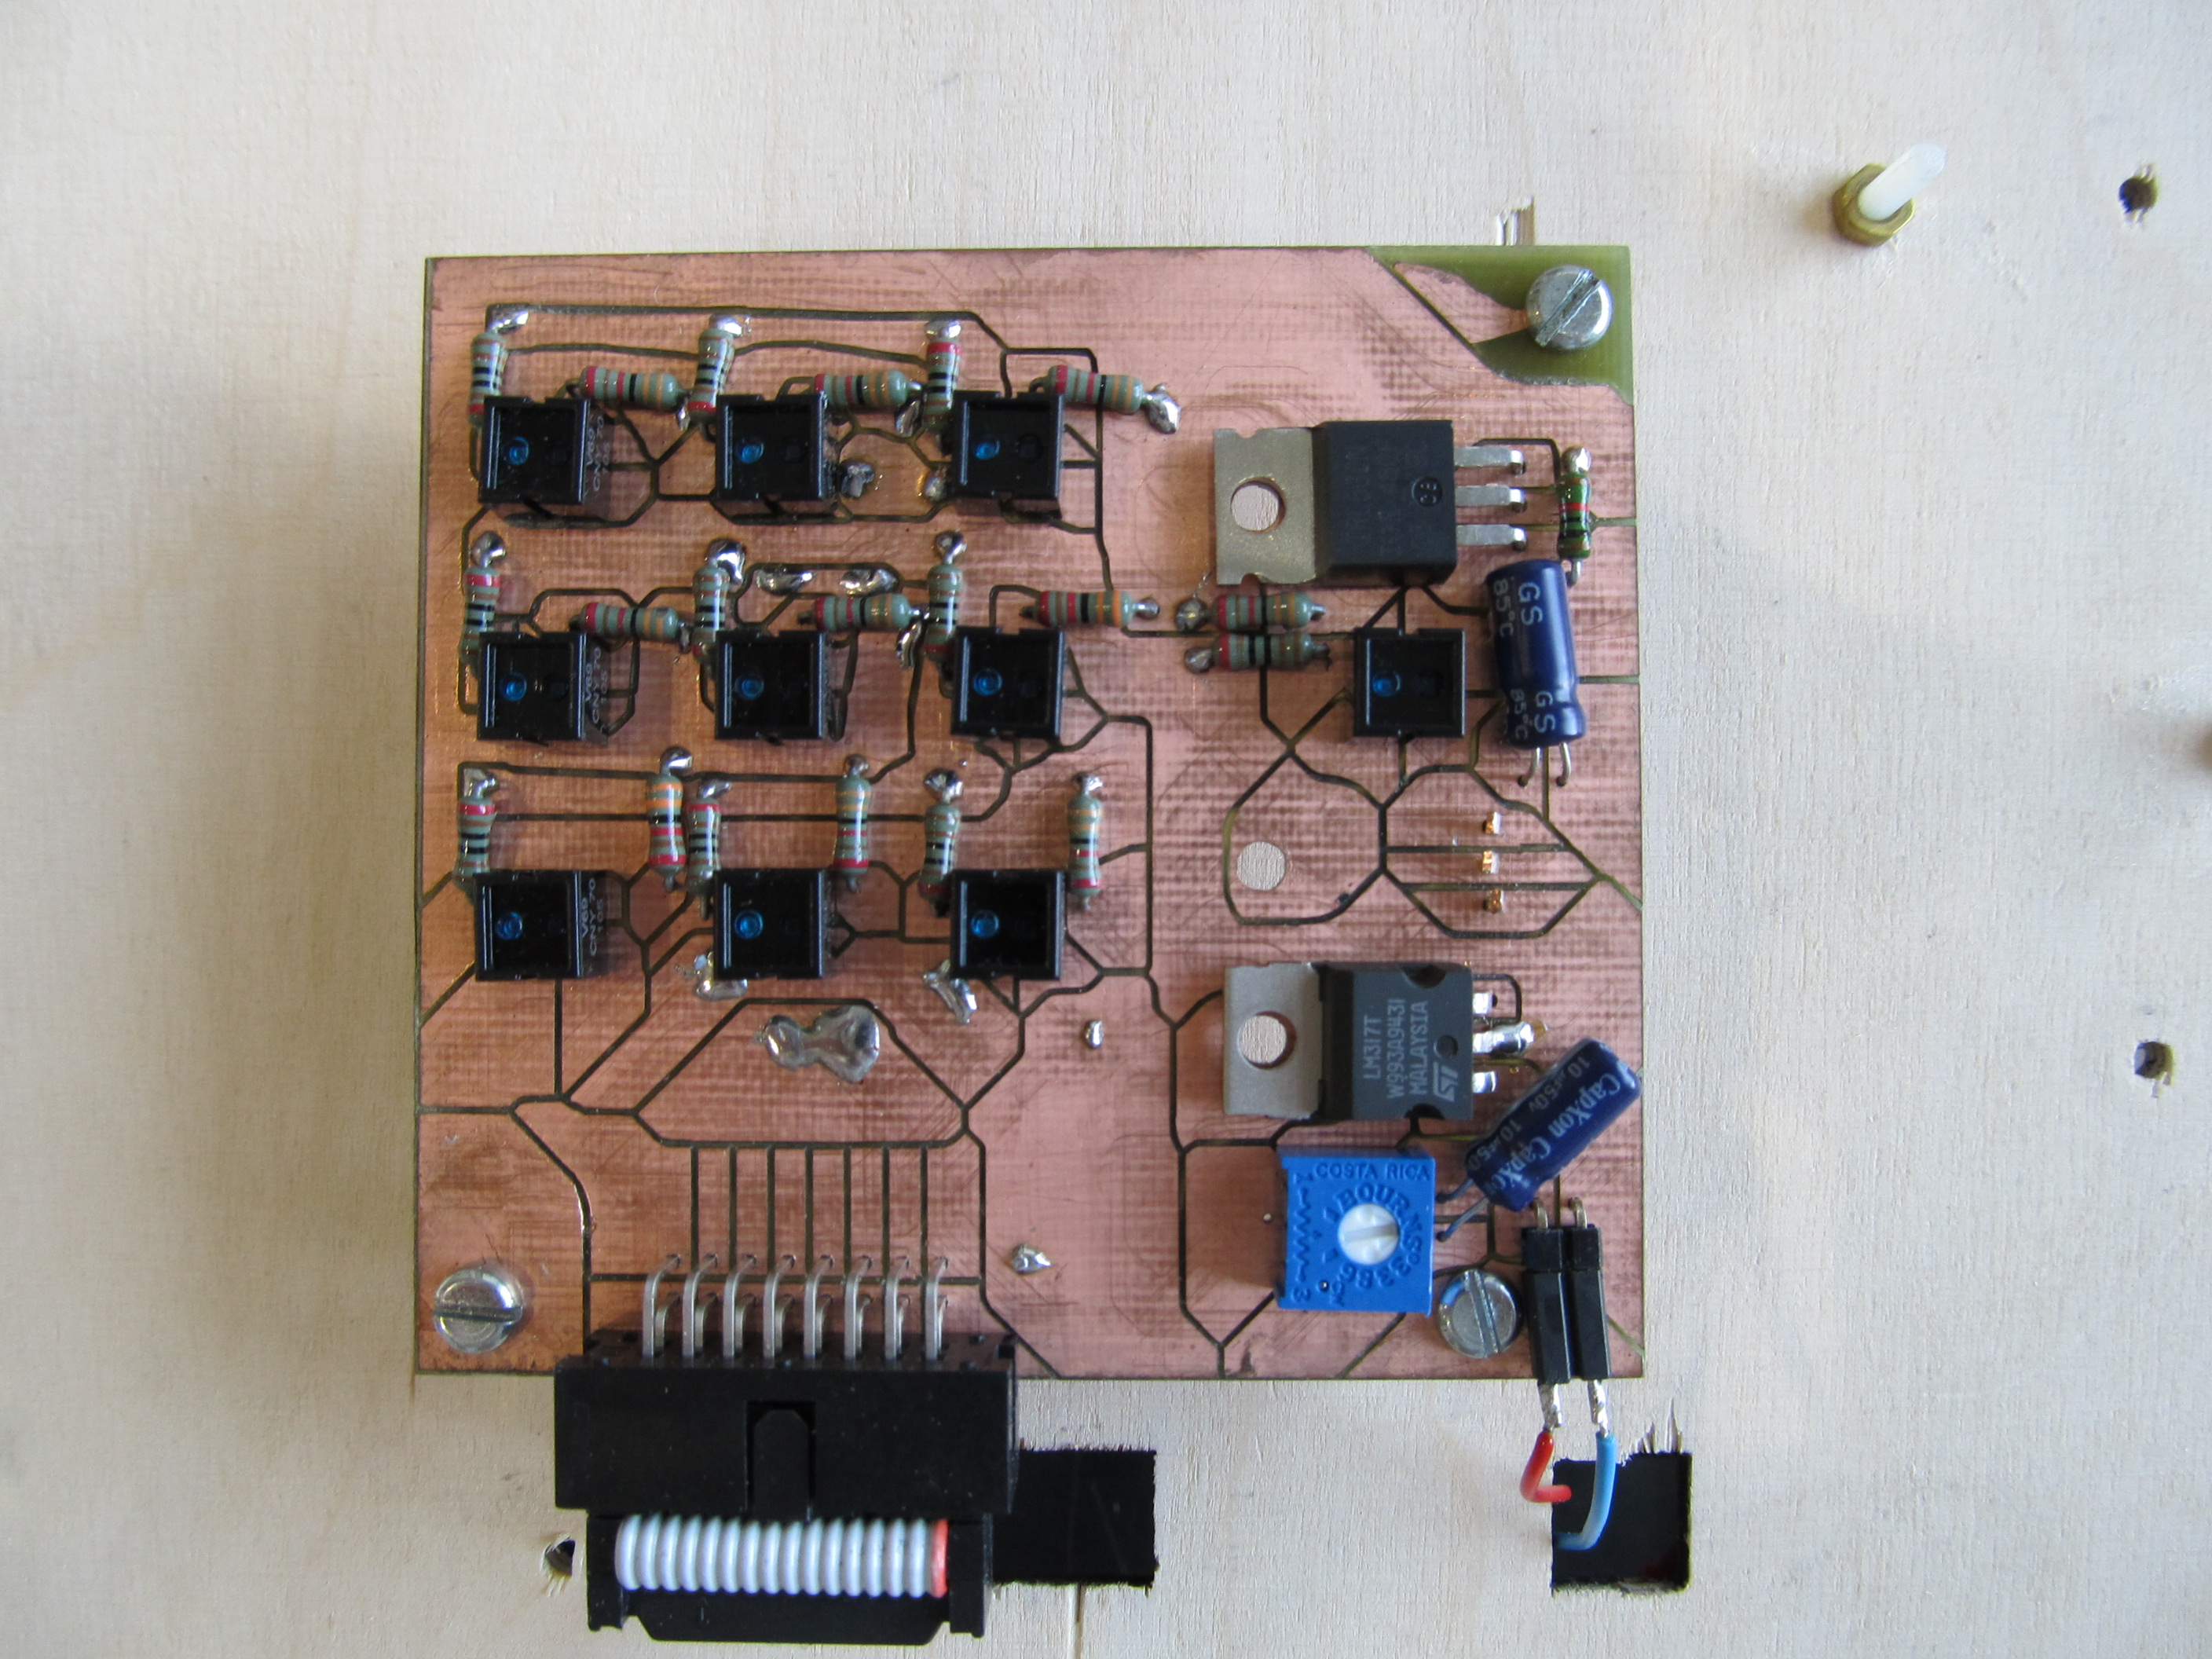
\includegraphics[width=125mm]{img/sensor_array.jpg}
\caption{Das unter dem Roboter montierte Sensorarrayt}\label{array3}
\end{figure}



\subsection{Spannungversorgung}\thispagestyle{empty}
Die Energie zum Betrieb des Roboters stammt aus einem Kokam 14,6V 4000mAh Litihum Lithium-Polymer-Akkumulator. Es wird empfohlen vor jeden Messzyklus den Akku zu laden. Ein voller Akku reicht für mehr als 10 Messfahrten. Der Akku ist mit einer im Anschlusskabel integrierten Schmelzsicherung geschützt. Zum Laden des Akkus muss der Akku vom Roboter abgesteckt werden und an das Ladegerät angeschlossen werden. Zum Schutz vor Kurzschlüssen ist der Akku mit einer im Anschlusskabel integrierten Schmelzsicherung gesichert. Zum Laden wird ein Ultramat 16 S verwendet, welcher alle vier Zellen des Akkus auf die gleiche Spannung lädt. 
Der Akku kann mit bis zu 200A belastet werden, allerdings liegt der maximale Strom aller 4 Motoren und der restlichen Elektronik liegt bei einem Ampere. Die Motoren werden direkt mit der Akkuspannung versorgt. Die Versorgungsspannung schwankt zwischen der vollen Akkuspannung 16,4V und 15V nach mehr als 10 Messfahrten.
Die 5 Volt Versorgung des Mikrocontrollers wurde mit einem RECOM R-785.0-1.0 DC-DC Konverter gelöst. Er ist pinkompatibel zu einem 7805, und bietet die Vorteile einer geringen Verlustleistung und einer sehr genauen Ausgangsspannung. 
Der Ladezustand der einzelnen Zellen des Akkus wird mit einer eigens dafür entwickelten Schaltung überwacht. Sollte die Spannung einer Zelle unter 3,3V sinken, wird die Stromversorgung zum Roboter mittels FET unterbrochen, und ein akustisches Warnung ausgegeben. Damit wird eine Tiefentladung verhindert, was zu einer irreversiblen Schädigung und einem Kapazitätsverlust führen kann. Eigentlich könnte der Akku bis zu 2,7V pro Zelle entladen werden (siehe Abbildung \ref{akku}.
\begin{figure}[htbp]
\centering
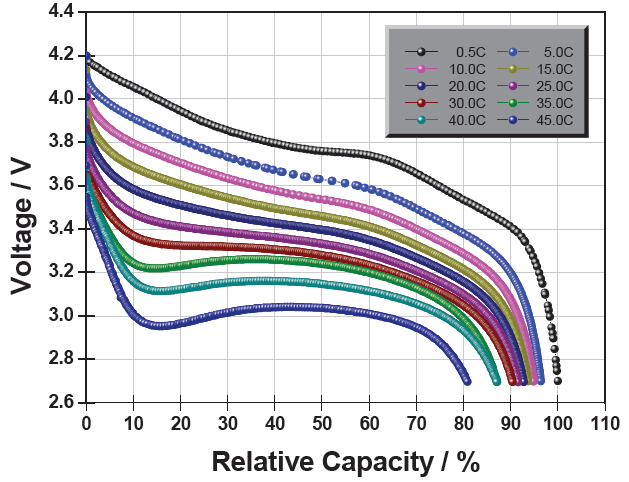
\includegraphics[width=100mm]{img/entladekurve.png}
\caption{Die Entladekurve einer Zelle des Akkus (1C = 4A).}\label{akku}
\end{figure} 
Die Analog-Digitalwandlung des Arduino benötigt eine Referenzspannung, entweder die Versorgungsspannung, was jedoch zu ungenau ist. Als Spannungsreferenz wird daher ein LT1021 5V Präzisionsspannungsquelle verwendet. Da dieses Bauelement nachträglich hinzugefügt wurde, ist es auf einer eigenen kleinen Platine untergebracht.

 
\subsection{Mikrokontroller}\thispagestyle{empty}
Der Arduino Mega 2560 ist ein Mikrocontroller-Board mit einem ATmega2560 Mikrokontroller. Es verfügt über 54 digitale I/O Pins, davon können 14 als PWM-Ausgänge verwendet werden. Weiters gibt es 16 analoge Eingänge die über einen 10-Bit Analog-Digital-Wandler verfügen.


\begin{figure}[htbp]
\centering
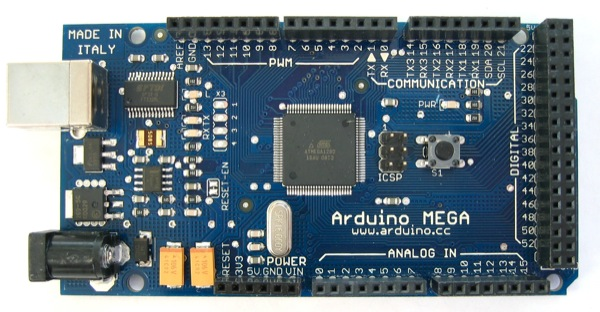
\includegraphics[width=100mm]{img/ArduinoMega.jpg}
\caption[Arduino Mega 2560]{Arduino Mega 2560}\label{ardu}
\end{figure}

\subsection{Temperatursensoren}\thispagestyle{empty}
Der Spannungsabfall an einem temperaturstabilen 100$\Omega$ Widerstand wird mit dem Spannungsabfall an einem PT100 verglichen. Als Stromquelle dient eine sehr präzise REF200-Stromquelle\cite{ref200}, welche zwei mal 100 Mikroampere $\pm$0.5$\%$ liefert. Abbildung \ref{tmess} zeigt den Schaltplan, Abbildung \ref{tmess2} zeigt das Platinenlayout.


\begin{figure}[htbp]
\centering
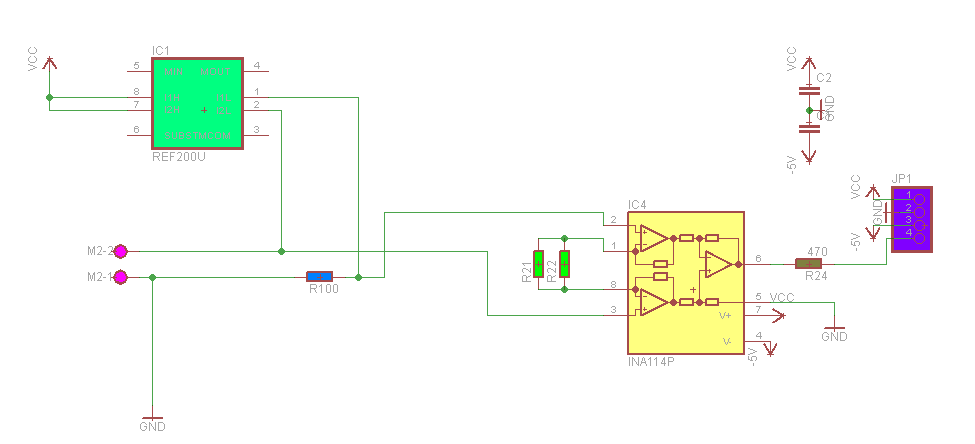
\includegraphics[width=125mm]{img/tmess.png}
\caption{Schaltung der Temperaturmessung}\label{tmess}
\end{figure}

\begin{figure}[htbp]
\centering
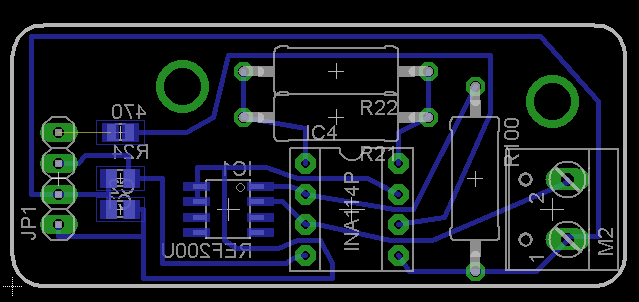
\includegraphics[width=100mm]{img/tmess2.png}
\caption[Arduino Mega 2560]{Layout der Temperarurmessung}\label{tmess2}
\end{figure}


\section{Softwareentwicklung}\thispagestyle{empty}
Dieser Abschnitt beschreibt die Entwicklung des Softwareteils. Es wird kurz auf die Entwicklungsumgebung eingegangen. Dann folgt die Auswertung der optischen Sensoren. Schließlich wird die Programmstruktur erklärt. Der gesamte Code ist im Anhang gelistet.

\subsection{Entwicklungsumgebung}\thispagestyle{empty}
Der Mikrocontroller auf den Arduino Board wird mit der Arduino Programmiersprache, welche auf Wiring basiert und sehr C-artig ist, in der Arduino Entwicklungsumgebung (siehe Abbildung \ref{ardu2}, welche auf Processing basiert, programmiert. Die Entwicklungsumgebung ist auf das notwendigste beschränkt, und erlaubt einen raschen Einstieg. Die umfassenden Beispielprogramme helfen beim Einarbeiten. Darüber hinaus gibt es eine große und aktive Comunity.
Ein Arduino Programm besteht aus zwei Teilen: Einer Setup-Routine die einmal zu Programmstart durchlaufen wird und einer Endlosschleife. In der Schleife wird das eigentlich Programm abgearbeitet. 

\begin{figure}[htbp]
\centering
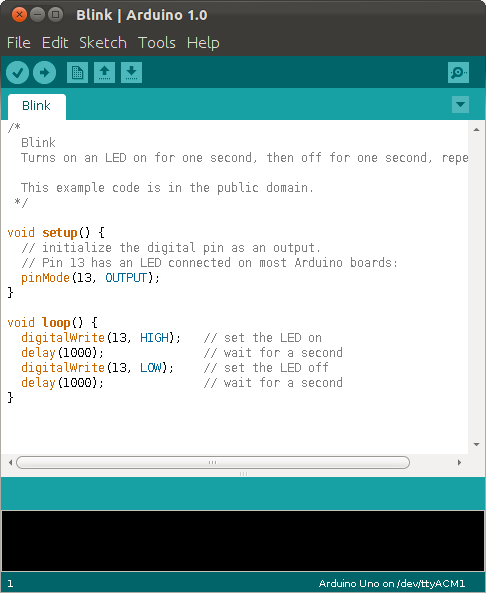
\includegraphics[width=100mm]{img/Arduino.png}
\caption[Die Arduino Entwicklungsumgebung]{Arduino Entwicklungsumgebung}\label{ardu2}
\end{figure}

\subsection{Auswertung der optischen Sensoren}\thispagestyle{empty}
Um den Einfluss des Streulichtes der starken Einstrahlung im Sonnensimulator auf die Optoreflektoren CNY70 zu vermeiden, wurde eine differentielle Messmethode angewandt. Die Messwerte bei ausgeschalteter Infrarot-Leuchtdioden werden von den Messwerten mit eingeschalteter Leuchtdioden abgezogen.
Das wird für alle neun Optoreflektoren des Sensorarray, sowie den Stopsensor, gemacht.
Mit den korrigierten Werten der einzelnen optischen Sensoren wird die Lage der Linie relativ zum Mittelpunktes des Arrays bestimmt. 

Die Höhe des Messwertes  der optischen Sensoren ist abhängig von der Helligkeit des Untergrundes. Unter der Annahme dass sich eine helle gerade Linie unter dem Senorarray befindet funktioniert folgende Formel:
\begin{align*}
  x_1 &= \frac{C-A}{2A-4B+2C} \\
  \\
  x_2 &=  \frac{F-D}{2D-4E+2F} \\
  \\
  x_3 &=  \frac{I-G}{2G-4H+2I} \\
  \\
  d &=  \frac{x_1+x_2+x_3}{3} \\
  \\
  k &=  \frac{x_1-x_3}{2}
\end{align*}


\begin{figure}
\centering
    \subfigure[Versatz]{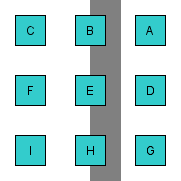
\includegraphics[width=50mm]{img/array5.png}}
    \subfigure[Verdrehung]{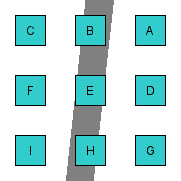
\includegraphics[width=50mm]{img/array6.png}}
\caption{Die mögliche Abweichungen der Linie von der Idealposition}
\end{figure} 


\subsection{Auswertung ADCs}\thispagestyle{empty}
Aufgrund von Rauschen der ADC-Werte, wurden alle Messwerte über 500 Einzelmessungen gemittelt. Die Quelle des Rauschens wurde nicht ermittelt. Der notwendige Messzeit dafür beträgt unter einer halben Sekunde. Die optischen Sensoren werden ebenfalls mit ADCs ausgewertet, die Behandlung erfolge im vorigen Unterabschnitt. 

\subsection{Programmablauf}\thispagestyle{empty}

\begin{figure}[htbp]
\centering
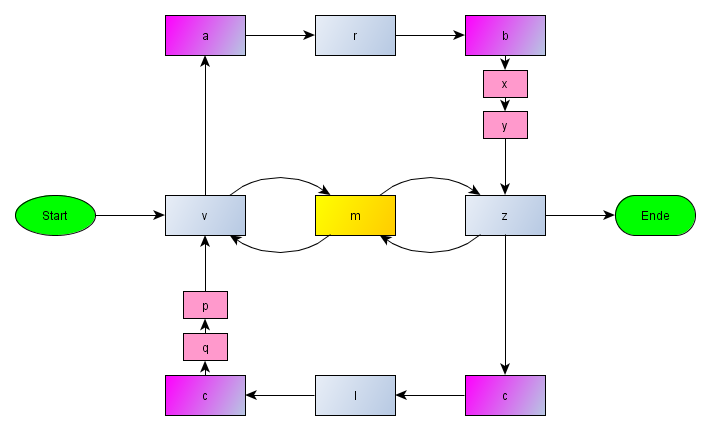
\includegraphics[width=150mm]{img/ablauf2.png}
\caption[Programmablauf]{Programmablauf}\label{abl}
\end{figure}

\begin{figure}[htbp]
\centering
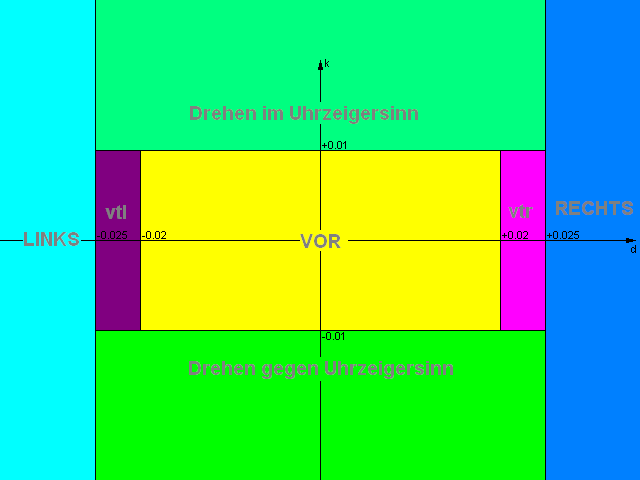
\includegraphics[width=75mm]{img/schranken.png}
\caption[Schranken der Regelung]{Schranken der Regelung}\label{schr}
\end{figure}

Das Programm startet im Modus Start, der Roboter steht, und wartet 60 Sekunden, eine Pufferzeit damit nach dem Einschalten des Roboters die Lade des Sonnensimulator hineingeschoben und die Klappe geschlossen werden kann.
Nach Ablauf dieser 60 Sekunden wechselt das Programm in den Modus Vorwärts. In diesem Modus fährt der Roboter in Vorwärtsrichtung. Abweichungen von der Idealspur werden erkannt und korrigiert. Wird mit dem Stopsensor eine Stopmarkierung erkannt, wechselt das Programm in den Messmodus. 
Ein Arduino Programm besteht grundsätzlich aus zwei Teilen: 
Eine Setup Routine, die einmal durchlaufen wird, und diverse Pins als Eingänge bzw. Ausgänge festlegt.
Eine so genannte Loop, die immer wieder durchlaufen wird, eine in der Loop integrierte Zeitverzögerung ist sinnvoll. 

Das Einschalten des Roboters ist der Start des Programms. Nach dem Start gibt es eine Verzögerung von 60 Sekunden, die dazu dient, die Einschublade des Sonnensimulators zu schließen. Es wird davon ausgegangen, dass der Roboter auf der Messbahn steht, das heißt das Senorarray befindet sich über der Messbahn.
Die gesamte Bewegungssteuerung ist als Zustandautomat ausgeführt. ( Ablauf2.png Bild der möglichen Zustände).
Mode s (Start): Zeitverzögerung von 60s, Übergang zu Mode v
Mode v (Vorwärtsfahrt) Mode z (Rückwärtsfahrt): Regelung zur Spurhaltung, Übergang zu Mode m (messen) bei erkannten Messpunkt, bei erkannter Ecke Übergang zu Mode a (Fahrt um die Ecke)
Mode a, Mode c: Eine um die Ecke Fahrt, bestehend aus zwei Einzelbewegungen: einer Geradeausfahrt bis die obere Sensorreihe (A, B und C) dunkel detektieren, gefolgt von einer Seitwärtsfahrt mit 700ms Dauer. (Funktionierende Lösung! Daher wurde keine Variante ohne Zeitverzögerung gesucht.)
Mode b, d: eine Fahrt der Dauer 850ms, in Richtung vor bzw. zurück, übergang in den Modus der Positionskorrektur (x \& y bzw q \& p).
Messmodus siehe unten. (Screenshot der Messdatei.)
Beendigung des Messmodus (Zustand m, Messen): Nach dem Speichern geht der Zustandsautomat wieder in den vorigen Bewegungsmodus über, dazu gibt es eine Hilfsvariable.

Ende der Messfahrt: Im Zustand z (und nur im Zustand z) wird das Ende der Linie als Übergangsbedingung in den Zustand e (=Ende) gewertet. 





Der Roboter beginnt nach Ablauf der Einschaltverzögerung seine Vorwärtsfahrt. (Bild mit den Bewegungsrichtungen des Roboters: vorwärts, rückwärts, links und rechts!)
Die Geradeausfahrt kann unterbrochen durch einen Messpunkte unterbrochen werden. Wenn der Messpunktsensor einen Wert höher als eine bestimmte Schaltschwelle erhält wird in den Messmodus gewechselt.
Messmodus: Zeitverzögerung um 250 ms, zur Vermeidung von elektromagnetischen Störungen durch die Motorströme. Messschleife von 500 Einzelmessungen des Zellenkurzschlussstromes, der Zelltemperatur und der Umgebungstemperatur. Die Einzelmesswerte werden zuerst summiert und nach der Schleife durch 500 dividiert. 
Schreiben auf SD Karte: Zeitpunkt in ms, zu dem die Messung gestartet hat, dann die 3 ADC Werte, Messpunkt, Messreihe und Messspalte. (Falls ein Messwert verloren geht, was vorkommen kann, wenn ein Messpunkt übersehen wird, kann die Position ermittelt und die fehlenden Messwerte geschätzt werden.

Die Messstrecke setzt sich aus geraden Linienelementen zusammen, die durch 90$\circ$ Ecken verbunden sind. Bei der Hälfte der Ecken ist die Linie nicht durchgehend, sondern als mit einem 15mm breiten Abstand ausgeführt. Das war nicht geplant, hat sich aber in der als funktionierende Lösung erwiesen. Das Seitwärtsfahren des Roboters funktioniert, aber es sind größere Abweichungen im Versatz und der Verdrehung möglich. Daher kann der Roboter in einer ziemlich ungünstigen Position an der Ecke stehen. Der Algorithmus des um die Ecke Fahrens besteht aus einer Fahrt (ohne Regelung!) in die bisherige Bewegungsrichtung solange bestimmte Sensoren des Arrays nicht dunkel detektieren, gefolgt von einer Bewegung von 90$\circ$ zur bisherigen Bewegungsrichtung ohne Regelung für eine definierte Zeit. Diese beiden Bewegungen können im schlimmsten Fall die ungünstige Position des Roboters so weit verschlimmern, dass eine Weiterfahrt nach der Ecke unmöglich ist.
Durch die Modifikation der Ecke, in ein Ende der Linie mit einem davon seitwärts versetzten Anfangs, vereinfacht sich der prinzipielle Algorithmus. Bis zum Ende der Linie ist es der normale (inkl. Regelung) Fahralgorithmus, danach wird 90$\circ$ zur bisherigen Bewegungsrichtung, d.h. vor oder zurück, mit einer definierten Zeit zur Überbrückung der Lücke ohne Regelung gefahren. Dann steht der Roboter auf der Linie, aber eventuell mit Versatz oder einer Verdrehung.

Regelung bei der Vorwärts bzw. Rückwärtsfahrt. A bei der Vorwärtsfahrt schwarz, G bei der Rückwärtsfahrt schwarz. Damit die Ecken keinen Einfluss (= ungewollte Verdrehung, wäre sehr schlecht als Ausgangslage für das um die Ecke fahren). Da es lange ohne Probleme funktioniert hat wird kein vermeidlich sinnloser Programmteil gelöscht. Die Auswirkungen sind nur durch lange Testfahrten zu ermitteln.
In der Regelung für das Fahren in Richtung "vor" gibt es neben der Bewegung für das Vorwärtsfahren noch 6 andere Bewegungsarten. Drehen am Stand mit und gegen den Uhrzeigersinn, links und rechtsfahren, und dann noch zwei Bewegungen die sich aus gleichzeitig drehen und vorwärts fahren zusammensetzen. Die Art der Bewegung ist von zwei Variablen dem seitlichen Versatz d und der Verdrehung k. Liegen beide Variablen innerhalb enger Grenzen fährt der Roboter geradeaus vor.
Für das Rückwärtsfahren ist die Regelung analog.

Unabhängig von der Regelung des Seitwärtsfahrens gibt es mechanische Kontaktelemente die eine zu starke Verdrehung des Roboters beim Seitwärtsfahrens gar nicht zulassen. Diese Kontaktelemente bestehen aus leichtem Schaumstoff und sind auf die Vorder- bzw. Rückseite des Roboters aufgeklebt.

Die Ecken müssen als solche erkannt werden, bevor sie die normale Fahrregelung stören.
Wird eine Ecke erkannt wird der normale Fahrmodus unterbrochen, und in einem speziellen Eckenmodus gewechselt.
Es gibt zwei Arten von Ecken: 
- einmal die klassische Ecke beim Wechsel vom Vor- bzw. Rückwärtsfahren nach rechts.
- Die nach Rechts-Fahren Bahn endet, anstatt in einer Ecke in die Vor- bzw. Rückwärtsbahn zu enden.
Damit ist auch das um die Ecke fahren auch unterschiedlich.
Im Vor- bzw. Rückwärts-Fahren wird die Fahrt ohne Regelung solange fortgesetzt bis die obere bzw. untere Zeile der Sensormatrix schwarz sieht, dann fährt der Roboter ohne Regelung einge hundert Millisekunden nach rechts. Erst dann wird in den nach Rechts-Fahr-Modus gewechselt.
Für den Rechts-fahr Modus endet die Linie abrupt. Der Roboter fährt einige hundert Millisekunden vor bzw. zurück. Dann steht er auf der Führungslinie. Bevor in den eigentlichen Vor- bzw. Rückwärtsfahrmodus gewechselt wird, wird der Roboter zur Linie hin ausgerichtet. Die Unterschiedliche Behandlung der Ecken ist notwendig, weil im Rechtsfahren größere Abweichungen von der Ideallinie auftraten als im Vor- und Zurückfahren.
Folge der Linie: Der Roboter fährt standardmäßig gerade aus. Wird ein Versatz zur Linie erkannt, wird dieser Versatz durch eine Bewegung normal zur Linie minimiert. Eine Verdrehung zur Linie wird durch Verdrehen des Roboters korrigiert. Ein minimaler Versatz, bzw. eine minimale Verdrehung ist dabei zulässig. 
Das vorwärts- und rückwärts-Fahren funktioniert dabei besser als das nach rechts-Fahren. Mecanum-Räder haben eine Vorzugsrichtung.
Haltepunkte: Haltepunkte werden mit dem Haltepunktsensor erkannt, wenn dieser den Schwellwert für weiß überschreitet. Damit ein Haltepunkt nicht mehrfach erkannt werden kann, gibt es eine Verriegelung in der Software, die einen neuen Haltepunkt erst wieder zulässt wenn der Haltepunktsensor in der zwischen Zeit schwarz gesehen hat.




\chapter{Kalibration}\thispagestyle{empty}

Dieses Kapitel beschreibt die Kalibrierung der Messsensoren. Es gibt drei Messplatinen, eine für die Messung des Kurzschlussstromes der Messzelle, und zwei identisch aufgebaute Messplatinen zur Messung der Zelltemperatur beziehungsweise der Umgebungstemperatur. Die Strom-Messplatine wandelt den Kurzschlussstrom der Messzelle in eine Spannung um, die in einem für den ADC des Arduino auswertbaren Bereich (0 bis 5 Volt) ist. Die beiden Messschaltungen zur Temperaturmessung wandeln die Größe der temperaturabhängigen Messwiderstände, jeweils ein Pt-100, in eine Spannung um.
Die ADC-Messwerte wurden über die USB-Schnittstelle des Roboters ausgelesen. Dafür benötigt der Roboter ein einfaches Kalibrierprogramm.



\section{Temperatursensoren}\thispagestyle{empty}
Die Temperatur der Messzelle wird mit einem von unten aufgeklebten flächigen Folienmesswiderstand gemessen. 
Ein zweiter Pt100, in kompakter Dünnschichtbauweise ausgeführt, misst die Temperatur der Umgebung. Beide Messskreise sind identisch aufgebaut, dennoch führen Bauteiltoleranzen zu leicht unterschiedlichen Verstärkungen.
Für die Kaltbration der Temperaturmesselektronik wurden die Pt-100 Widerstände durch einen hoch genaues, einstellbares und kalibriertes Messnormal ersetzt. Der Widerstand wurde im Bereich von 100 bis 122 	$\Omega$  in 1 $\Omega$  Schritten verändert, was einer Temperatur von 0 bis 55 $^{\circ}$C entspricht. Die ADC-Werte wurden über die USB-Schnittstelle des Arduino ausgelesen. Es zeigte sich, dass die beiden Schaltungen leicht unterschiedliche Verstärkungen haben. Daher mussten jede Temperaturmessschaltung separat kalibriert werden.

\begin{table}[htbp]
\centering
\begin{tabular}{ | c | c | }\hline
{\bf R / $\Omega$ } & {\bf ADC Wert}\\ \hline
\hline
101 & 12\\ \hline
102 & 53\\ \hline
103 & 93\\ \hline
104 & 133\\ \hline
105 & 173\\ \hline
106 & 212\\ \hline
107 & 253\\ \hline
108 & 293\\ \hline
109 & 332\\ \hline
110 & 374\\ \hline
111 & 412\\ \hline
112 & 454\\ \hline
113 & 493\\ \hline
114 & 533\\ \hline
115 & 573\\ \hline
116 & 613\\ \hline
117 & 653\\ \hline
118 & 694\\ \hline
119 & 734\\ \hline
120 & 775\\ \hline
121 & 815\\ \hline
122 & 857\\ \hline
\end{tabular}
\caption{Die Messwerte der Kalibrierung Messschaltung A}\label{TabA}
\end{table}

Obwohl der 10-Bit ADC des Arduino einen Maximalwert von 1023 hat, ist bedingt durch den Einsatz des Instrumentenverstärkers INA114, der maximale ADC-Wert bei 857, was einer Spannung von 4,18V entspricht.  


\begin{figure}[htbp]
\centering
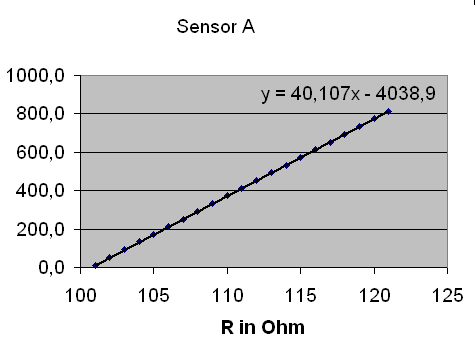
\includegraphics[width=100mm]{img/messa.png}
\caption{Ausgleichsgerade Temperaturmessung A}\label{messa}
\end{figure}

\begin{table}[htbp]
\centering
\begin{tabular}{ | c | c | }\hline
{\bf R / $\Omega$ } & {\bf ADC Wert}\\ \hline
\hline
100 & 0\\ \hline
101 & 20\\ \hline
102 & 60\\ \hline
103 & 99\\ \hline
104 & 139\\ \hline
105 & 179\\ \hline
106 & 219\\ \hline
107 & 259\\ \hline
108 & 299\\ \hline
109 & 339\\ \hline
110 & 379\\ \hline
111 & 420\\ \hline
112 & 460\\ \hline
113 & 499\\ \hline
114 & 539\\ \hline
115 & 579\\ \hline
116 & 619\\ \hline
117 & 659\\ \hline
118 & 700\\ \hline
119 & 740\\ \hline
120 & 780\\ \hline
121 & 820\\ \hline
122 & 857\\ \hline
\end{tabular}
\caption{Die Messwerte der Kalibrierung Messschaltung B}\label{TabB}
\end{table}

\begin{figure}[htbp]
\centering
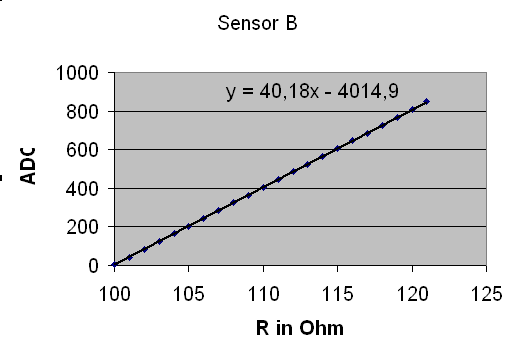
\includegraphics[width=100mm]{img/messb.png}
\caption{Ausgleichsgerade Temperaturmessung B}\label{messb}
\end{figure}

Die mit Excel gewonnen Gleichungen der Ausgleichsgerade für Messschaltung A (siehe Abbildung ~\ref{messa}) und B (siehe Abbildung ~\ref{messa}) werden verwendet um aus den ADC-Werten die dazugehörigen Widerstandswerte zu berechnen. 

  \begin{equation}
     R_A(ADC) = \frac{ADC_A + 4039,9}{40,107}
  \end{equation}
  
    \begin{equation}
     R_B(ADC) = \frac{ADC_B + 4023,6}{40,027}
  \end{equation}


\section{Messzelle}\thispagestyle{empty}


Der Kurzschlussstrom der Messzelle wurde im Flasher (siehe Abbildung~\ref{zelleflasher}) über einen weiten Temperaturbereich gemessen (siehe Abbildung~\ref{tempkoef}). Es wurde mit der Berger Messlast \cite{berger} gemessen. Bei der Messung wurden die Leitungswiderstände der Messkabel minimiert, indem Kabel mit hohem Querschnitt (6mm$^2$) verwendet wurden, und die Kabel möglichst kurz gehalten wurden (<1,5m).
 
\begin{figure}[htbp]
\centering
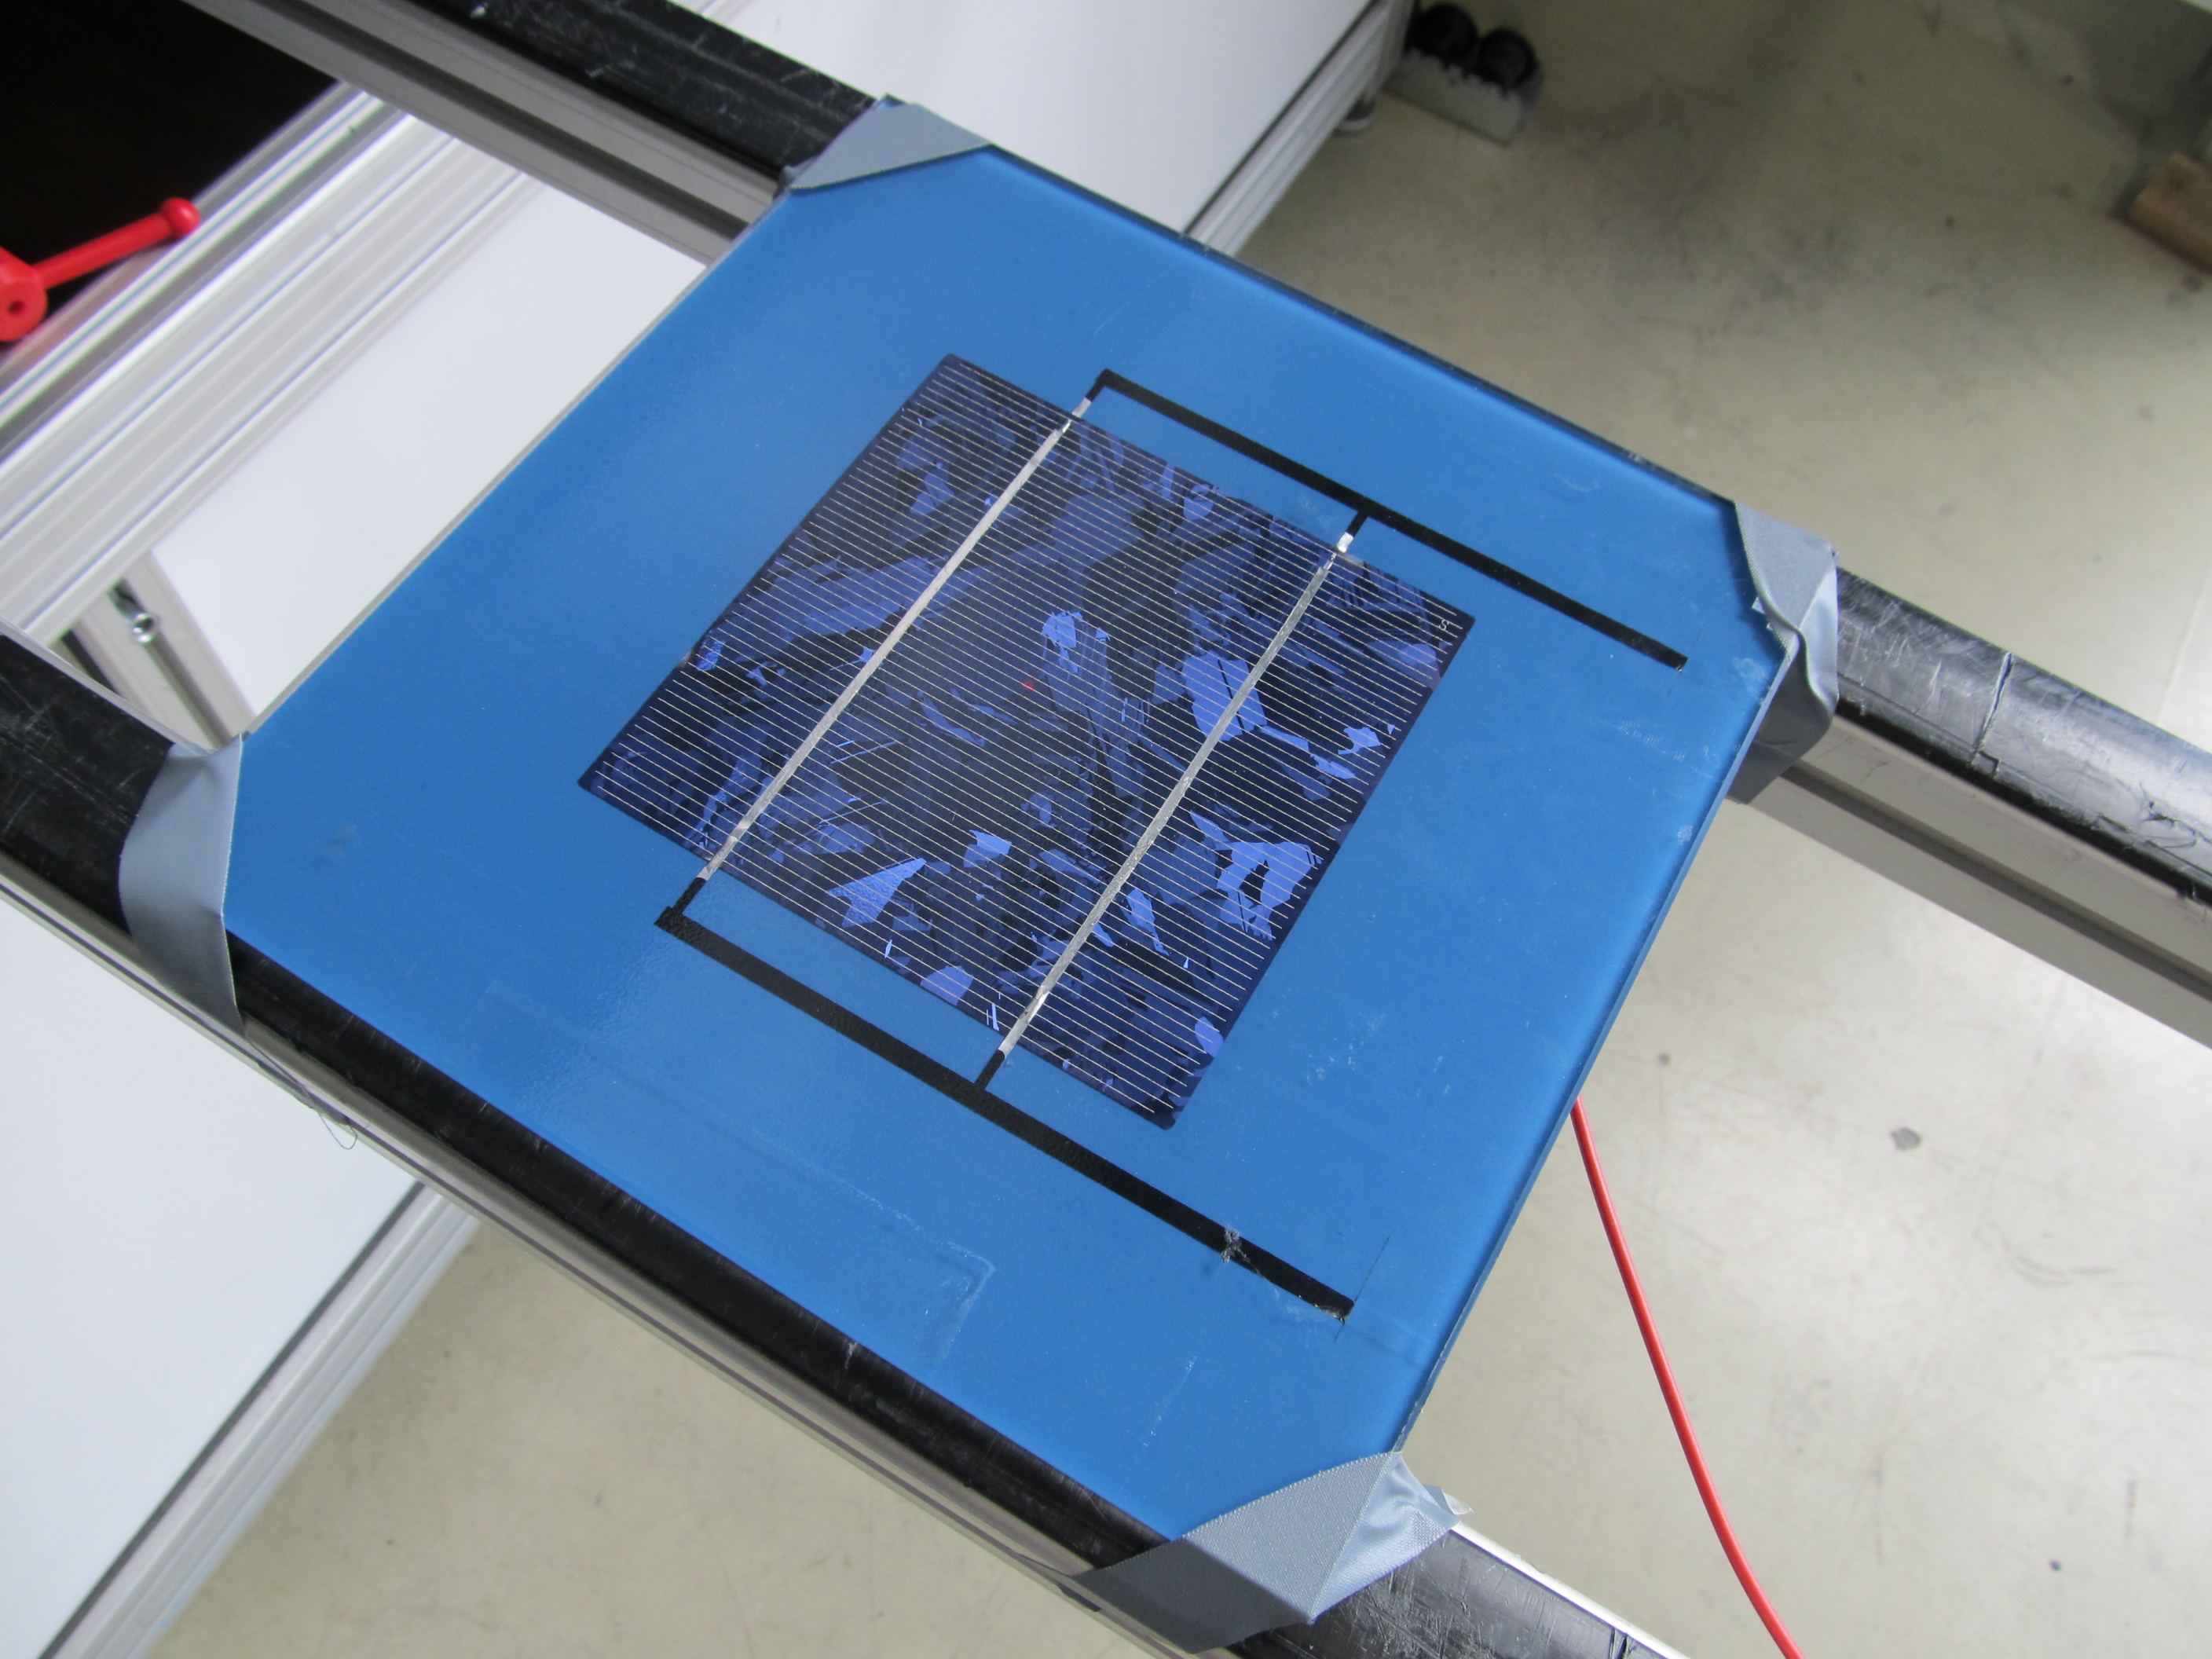
\includegraphics[width=75mm]{img/zelle.jpg}
\caption{Ein Photo der Messzelle}\label{zelleflasher}
\end{figure}

\begin{figure}[htbp]
\centering
\includegraphics[width=150mm]{img/Isc.png}
\caption{Abhängigkeit des Kurzschlussstromes von der Temperatur}\label{tempkoef}
\end{figure}

  \begin{equation}
     I(T) = 4,9529+0.0024 \ast T
  \end{equation}
  
    \begin{equation}
     I(T) = 4,9529 \ast ( 1 + 0,00048 \ast T)
  \end{equation}

\section{Strommessung}\thispagestyle{empty}

Der Messroboter wurde für die Kalibrierung der Strommessung in eine Klimazelle platziert.  Die Temperatur der Klimazelle wurde im Bereich von 8 bis 35 $^{\circ}$C variiert. Durch den Messwiderstand der Strommessung wurde ein Strom im Bereich von 3 bis 8 A geschickt.  

\begin{table}[htbp]
\centering
\begin{tabular}{|l|l|l|}
\hline
T/$^{\circ}$C & I/mA & ADC Wert \\ 
\hline
\hline

\multirow{3}{*}{24,4} & 3997 & 472 \\
 & 6001 & 712 \\
 & 8002 & 854 \\ \hline
\multirow{3}{*}{35,3} & 3999 & 473 \\
 & 6001 & 712 \\
 & 7999 & 859 \\ \hline
\multirow{3}{*}{35,3} & 3999 & 472 \\
 & 6001 & 710 \\
 & 8001 & 852 \\ \hline
\multirow{5}{*}{16,4} & 2004 & 234 \\
 & 3005 & 353 \\
 & 4003 & 473 \\
 & 5003 & 591 \\
 & 6005 & 711 \\ \hline
\multirow{5}{*}{8} & 1993 & 233 \\
 & 2995 & 352 \\
 & 4001 & 472 \\
 & 5000 & 590 \\
 & 6005 & 710 \\ \hline
\end{tabular}
\caption{Kalibrierung Strommessung}\label{TabS}
\end{table}

\begin{figure}[htbp]
\centering
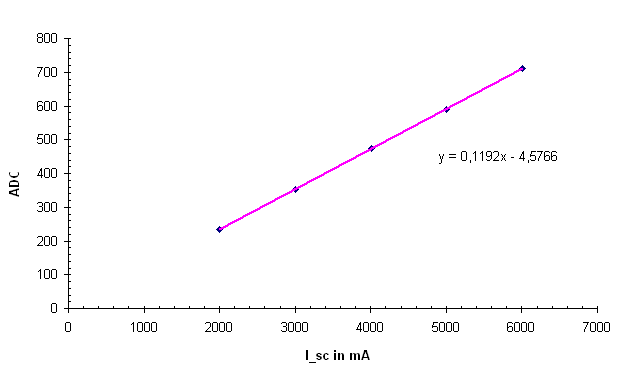
\includegraphics[width=150mm]{img/16grad.png}
\caption{Lineraer Zusammenhang zwischen Strom und dem ADC-Wert}\label{ical}
\end{figure}

\begin{equation}
     I(ADC) = \frac{ADC + 4,5766} {119,2} 
\end{equation}
  


\section{Thermische Stabilität der Temperaturmessung}\thispagestyle{empty}
Zur Bestimmung der Temperaturstabilität wurde der gesamte Roboter in ein Klimakammer gestellt. Der Pt100 wurde durch einen temperaturstabilen 110$\Omega$ simuliert.
Es gab zwei Durchgänge dieses Versuches.
Bei der ersten Messung zeigte sich, dass eine der beiden Messplatinen nicht temperaturstabil war. Durch das Tauschen der Ref200 Stromquelle dieser Platine konnte das Problem gelöst werden.

\begin{table}[htbp]
\centering
\begin{tabular}{ | c | c | c |}\hline
{\bf T / $^{\circ}$C} & {\bf ADC Platine A} & {\bf ADC Platine B}\\ \hline
\hline
11,7 & 368 & 407\\ \hline
13,0 & 368 & 406\\ \hline
13,7 & 368 & 406\\ \hline
14,5 & 368 & 405\\ \hline
15,5 & 368 & 405\\ \hline
16,6 & 368 & 405\\ \hline
17,5 & 368 & 404\\ \hline
23,5 & 368 & 403\\ \hline
27,5 & 368 & 402\\ \hline
\end{tabular}
\caption{Temeraturabhängigkeit der Temperaturmessung}\label{TabT1}
\end{table}

\begin{table}[htbp]
\centering
\begin{tabular}{ | c | c | c |}\hline
{\bf T in $^{\circ}$C} & {\bf ADC Platine A} & {\bf ADC Platine B}\\ \hline
\hline
30,7 & 368 & 380\\ \hline
20,1 & 368 & 379\\ \hline
9,2 & 368 & 378\\ \hline
\end{tabular}
\caption{Temeraturabhängigkeit der Temperaturmessung}\label{TabT2}
\end{table}

Durch den Austausch der Referenzstromquelle der Platine B hat sich auch der ADC-Wert gegenüber der ersten Messung geändert. Die Kalibrierwerte der Platine B \ref{TabB} sind nach diesem Austausch aufgenommen worden.
Da die Platine A temperaturstabiler als die Platine B ist, wurde Platine A zur Messung der Zelltemperatur ausgewählt, die Platine B wurde für die Messung der Umgebungstemperatur verwendet. 

\chapter{Messung}\thispagestyle{empty}

Diese Kapitel beschreibt die Messvorbereitung, den Messaufbau, die eigentliche Messung und die Auswertung der Messdaten. Um was geht es? Um die Messung. Zur Messung gehört der Messaufbau, der Messablauf und die Auswertung der Messung. Weiters werden Messungen bei verschiedenen Einstellungen diskutiert. 

\section{Messaufbau}\thispagestyle{empty}
Dieser Abschnitt behandelt den Messaufbau. Die Messung der Bestrahlungsstärkeverteilung findet im Sonnensimulator statt. Zuerst muss eine Messebene geschaffen werden. Die, im normalen Messalltag vermessenen, Module liegen auf verschiebbaren Metallschienen auf. Damit der Roboter fahren kann, braucht er eine ebene Fläche. Diese Fläche ist aus logistischen Gründen aus drei einzelnen Holzplatten gebildet, was einige zusätzliche Probleme bereitet hat. Auf der Oberseite der Platten befindet sich die Messpunkte und eine Führungslinie, welcher der Roboter folgt. Zur Messung wird der Roboter an das linke Ende der Linie gestellt, er fährt nach dem Einschalten selbständig das Messprogramm ab.

\begin{figure}[htbp]
\centering
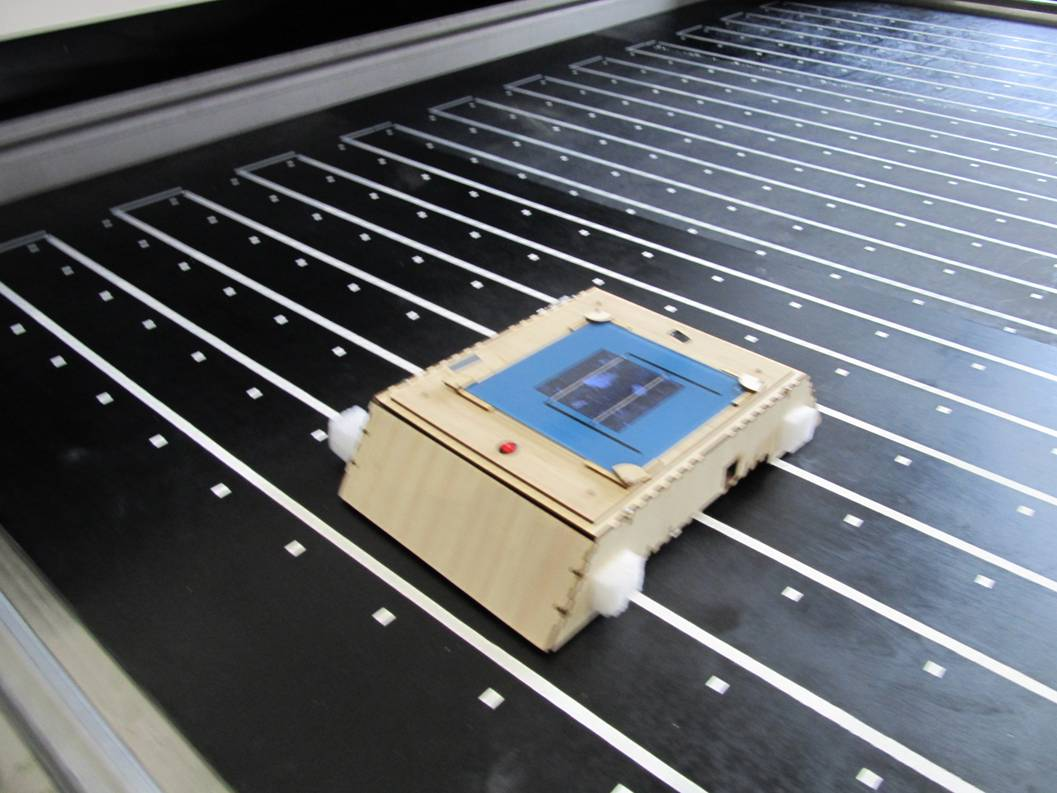
\includegraphics[width=100mm]{img/robofahrt.jpg}
\caption{Eine Fahrt des Roboters auf der Messbahn}\label{robofahrt}
\end{figure}

  \subsection{Platten}\thispagestyle{empty}
Drei Holzplatten bilden die Messebene für den Roboter. Eine große Platte wäre eine bessere Alternative gewesen, aber aus logistischen Gründen ist die Messebene auf drei Platten aufgeteilt. Weil für die drei Platten leichter ein Platz zum Aufbewahren gefunden werden kann. Die 250 mal 125 Zentimeter großen und 18 Millimeter dicken Holzplattenlatte sind gerade noch hantierbar. 
Die Platten sind schwarz, damit sie einen möglichst geringen Reflexionskoeffizienten haben. Um einen großen Unterschied im Reflexionskoeffizienten zu haben, ist die Messbahn weiß gehalten. Sowohl der schwarze Untergrund als auch die weiße Bahn ist mit Kunstharzfarbe ausgeführt. Beim Hantieren mit den Platten können kleine Beschädigungen der Messbahn entstehen. Da diese Beschädigungen  den Messablauf stören können, ist es ratsam vor der Messung die Bahn mit einem weißen Klebeband (Isolierband) auszubessern.
Die Platten müssen eng aneinander anliegen, damit der Roboter von einer Platte zur anderen fahren kann. Damit keine zu groß Stufe wegen unterschiedlicher Duschbiegung der Platten entsteht ist auf der Rückseite der Holzplatten Aluminiumbleche befestigt, auf einer Seite angeschraubt, die danebenliegende Platte liegt darauf.
Da die Breite aller 3 Platten geringer ist als die Breite der Lade des Sonnensimulators, werden, damit die Messungen zu verschiedenen Zeitpunkten verglichen werden können, die Platten so weit wie möglich nach rechts geschoben. Am Rand liegen die Platten auf Aluschienen auf.
Die Messpunkte liegen im Raster von 15 Zentimeter. Die Führungslinie 25,4 Millimeter daneben, gemessen vom Zentrum des Messpunktes zur Mitte der Linie. Die Messpunkte sind kleine Quadrate der Seitenlänge von 14 bis 15 Millimeter. Die Messbahn ist ebenfalls 14 bis 15 Millimeter breit. Die Position der Messpunkte ist auf etwa ein bis zwei Millimeter genau.
Die Messpunkte liegen im Abstand von 15 cm, damit ist auch der Abstand zwischen den Messbahnen 15 cm, der Roboter muss nur 15 cm seitwärts fahren. Die Übergänge der Messbahn von einer Platte zur nächsten sind mit weißem Isolierband  der Breite 14 Millimeter zu überbrücken. Beschädigung der Messbahn, welche durch unsanftes Handling der Platten entstehen können, sind ebenfalls mit weißem Isolierband zu Überkleben.
Die Messebene wird aus 3 Holzplatten gebildet, diese sind auf der Oberseite schwarz gefärbt und mit einer weißen mäanderförmigen Spur versehen. Die Platten hängen durch, dadurch ist die Messebene nicht eben. Schlimmer ist der nicht gleiche Durchhang verschiedener Platten. So kommt es zu einem Höhenunterschied zwischen den Platten. Um diese Stufen zu verringern wurde auf der Unterseite der Platten mit dem geringeren Durchhang eine kleine Aluplatte befestigt um eine Auflage für die andere Platte zu schaffen. Eine zu große Stufe behindert den Roboter beim Fahren. Weil an der Stufe nicht alle Haltepunkte zuverlässig erkannt werden können.


\begin{figure}[htbp]
\centering
\includegraphics[width=125mm]{img/messbahn1.png}
\caption[Messbahn auf den Platten]{Messbahn auf den Platten}\label{bahn}
\end{figure}






\subsection{Ablauf}\thispagestyle{empty}
Vor der Messung ist der Akku des Roboters voll zu laden. Der roboter ist auf mechanische Beschädigung zu Untersuchen, eventuell ist ein Rad locker, dann lässt es sich entlang der Achse verschieben.
Zuallererst sind die Platten auf Beschädigung zu untersuchen. Beschädigungen der Messbahn sind mit einem weißen Isolierband zu überkleben. Beschädigungen des Holzes direkt neben der Messbahn sind mit schawrzer Farbe auszubessern. Stellen, die der Sensor nicht sehen kann, sind egal.
Die Platten sind in den Einschub des Sonnensimulators zu legen. Das ist ein Puzzle und nicht schwer. Beginnend rechts. Die Übergänge der Messbahn von einer Platte zur nächsten sind mit weißem Isolierband  der Breite 14mm zu überbrücken. Beschädigung der Messbahn, welche durch unsanftes Handling der Platten entstehen können, sind ebenfalls mit weißem Isolierband zu Überkleben.



Roboter wird auf das linke vordere Ende der Messbahn gestellt. Der Roboter muss dabei auf der Messbahn stehen. Kleinere Abweichungen der Idealposition werden beim losfahren korrigiert. 
Vor der eigentlichen Messfahrt ist eine Testfahrt mit geöffneter Lade des Sonnensimulators zu empfehlen. Besonders die Übergänge von einer Platte zur nächsten können Probleme schaffen.
Nach der bestandenen Testfahrt wird der Sonnensimulator eingeschaltet. Bis zur Messung sind 20 bis 30 Minuten zu warten, bis die Temperaturen im Simulator stabil sind. Der Roboter kann während dieser Zeit im Sonnensimulator stehen. Die Messzelle sollte allerdings abgeschattet werden, damit diese sich nicht aufheizt. 
Zum Starten wird der Schalter von 0 auf 1 umgelegt. Damit wird der Mikrocontroller mit Spannung versorgt. Das Programm startet. Nach einer Pause von 60 Sekunden, die zum Schließen des Sonnensimulators notwendig ist, fährt der Roboter los. Eine Messfahrt dauert etwa 13 Minuten. Nach Ablauf dieser Zeit wird der Roboter entnommen und die Daten der SD-Karte entnommen, oder der Roboter wird auf die Startposition gestellt um weitere Messfahrten durchzuführen.


\section{Auswertung}\thispagestyle{empty}


Die Messwerte werden auf SD-Karte als Textdatei gespeichert. Für jeden Messwert gibt es eine eigene Zeile. In jeder Zeile sind Messzeit in Millisekunden, der ADC-Wert für den Kurzschlussstrom, der ADC Wert für die Zelltemperatur, der ADC Wert für die Umgebungstemperatur, und jeweils einen Zählerwert für Messpunkt, Reihe und Spalte. Die einzelnen Werte sind durch einen Tabulator getrennt, damit ist die Datei in Excel und Matlab bearbeitbar.  

Die Tabelle \ref{TabSD} zeigt wie die Daten auf der SD-Karte gespeichert sind. Es sind nicht alle Werte für die Auswertung notwendig. Der Erste Wert ist die Zeit in Millisekunden, die seit dem Einschalten des Roboters vergangen ist. Die nächsten 3 Werte sind werte des Analogdigtalwandlers im Bereich von Null bis 1023, diese Werte werden ohne Umrechnung direkt auf die SD Karte gespeichert. Es sind 308 Messpunkte, 14 mal 22, es kann vorkommen, am Übergang von einer Platte zur anderen, dass ein Messpunkt ausgelassen wird. Das ist erkennbar wenn nicht 308 Messwerte im datalog-File sind. Um den Fehler leicht zu finden wurde Spalte und Reihe mit aufgezeichnet. Sind in einer Spalte nur 13 Messwerte, fehlt in dieser Spalte ein Wert. Anhand der mit aufgezeichneten Zeit kann der fehlende Messpunktes lokalisiert werden. Das geschieht nicht automatisch Der Messwert wird anhand der neben liegenden Werte geschätzt. Alternativ werden nur Messfahrten mit allen Punkten ausgewertet.
 
\begin{table}[htbp]
\centering
\begin{tabular}{ | c | c | c | c | c | c | c | } 
\hline
$\frac{t}{ms}$ & I$_{SC}$ & T$_{Zelle}$ & T$_{Umgebung}$ & Messpunkt & Messpunkt 2 & Messreihe \\
\hline
\hline
{165515} & {466} & {437} & {237} & {47} & {5} & {4} \\
\hline
{167523} & {479} & {437} & {235} & {48} & {6} & {4} \\
\hline
{169551} & {471} & {437} & {228} & {49} & {7} & {4} \\
\hline
\end{tabular}
\caption{Ein Ausschnitt der Messwertedatei}\label{TabSD}
\end{table}

Im Zuge der Auswertung wird ein eindimensionales Array von 308 Messwerten in ein zweidimensionales Array von 14 mal 22 Zahlen umgewandelt. Dazu wird der erste bis zum 14. Wert des eindimensionalen Arrays zur ersten Reihe des zweidimensionalen Arrays. Der 15. bis zum 28. Wert des eindimensionalen Arrays bilden die zweite Reihe des zweidimensionalen Arrays, allerdings in umgekehrter Reihenfolge. So bildet die Reihenfolge der Messwerte des zweidimensionalen Arrays die Messfahrt des Roboters ab.
\newline

\begin{equation}
\begin{pmatrix}
n_1 \\ . \\ . \\ . \\ n_{308} 
\end{pmatrix}
\Longrightarrow
\begin{pmatrix}
n_{1}  & . &.& .& n_{14} \\
n_{28} & .& .& . &n_{15}  \\
n_{29}  &. &.& .& n_{42}  \\
. &.& .& . & . \\
n_{295}  &.& .&.& n_{308} 
\end{pmatrix}
\end{equation}

Um die eindimensionale Datenwurst Datenwurst in ein zweidimesionales Array, das der realen Anordnung der Messpunkte entspricht, wird folgender Algorithmus verwendet:
\begin{verbatim}
j=1; k=1; l=1;

for(i=0:307)
    if(mod(i,28)>13) k = 28- mod(i,28);
    else k = mod(i,14)+1;
    end
    B(k,l)=A(i+1);
    if(mod(i+1,14)==0) l=l+1;
    end
end
\end{verbatim}

Beschreibung verbal: Es gibt 308 Messwerte. Die ersten 14 werden in die erste Reihe des Arrays gelegt. Die nächsten 14 in die zweite Reihe, aber in in absteigender Reihenfolge. Das heißt in die 14. Spalte der 2. Reihe wird der 15 Wert gelegt, also erste Reihe von links nach rechts, die zweite Reihe von rechts nach links, die dritte Reihe wieder von links nach rechts, usw.







Der ADC Wert des Kurschlussstromes wird in Ampere umgerechnet. Verwendet wird dazu die in im Abschnitt Kalibrierung gewonnene Formel.

\begin{figure}[htbp]
\centering
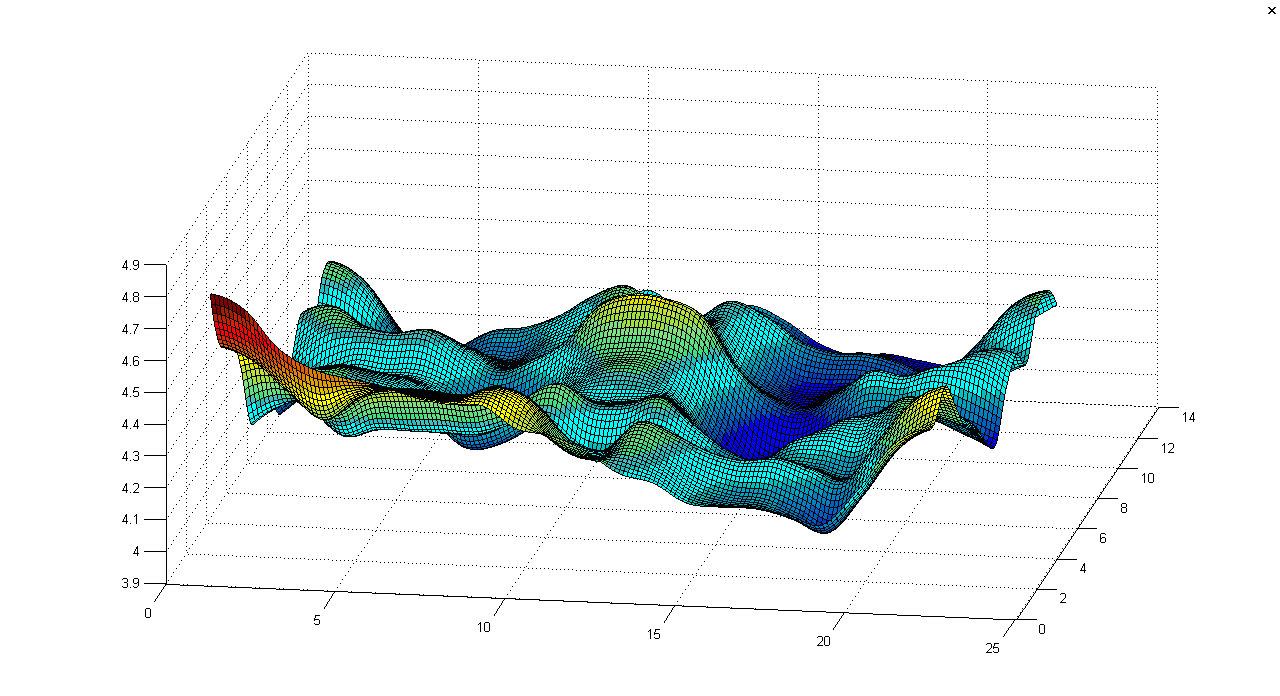
\includegraphics[width=150mm]{img/hugel.png}
\caption[Kurzschlusstromes in Ampere]{Verteilung des Kurzschlusstromes in Ampere abhängig von der Position}\label{hugel}
\end{figure}



\begin{figure}[htbp]
\centering
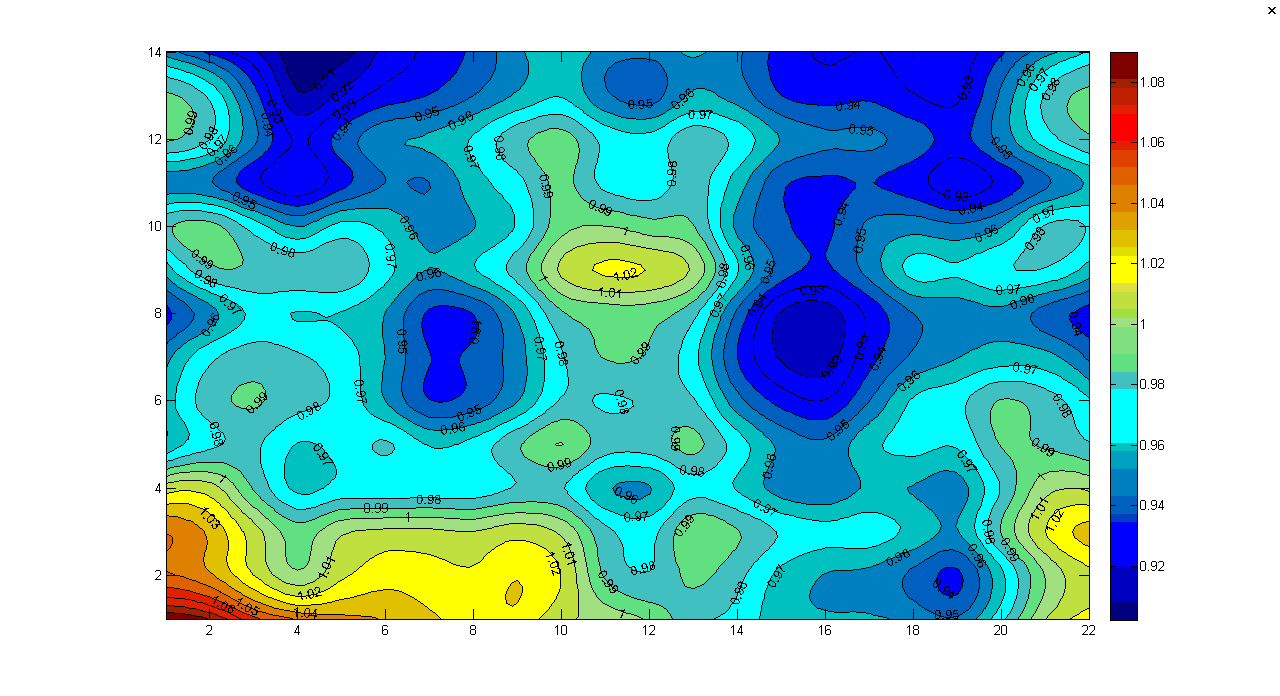
\includegraphics[width=150mm]{img/karte1.png}
\caption[Relative Verteilung der Einstrahlung]{Relative Verteilung der Einstrahlung}\label{karte1}
\end{figure}

\begin{figure}[htbp]
\centering
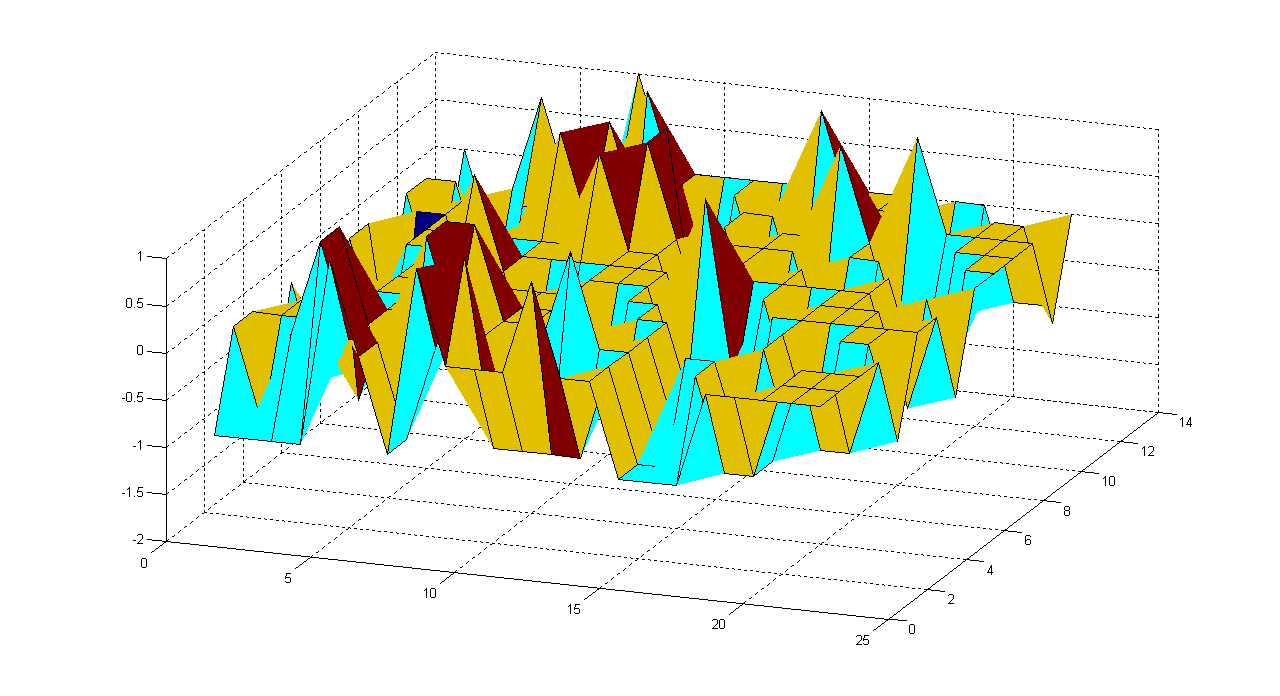
\includegraphics[width=150mm]{img/vergleich23.png}
\caption{Vergleich zweier Messungen}\label{vergleich}
\end{figure}

\begin{figure}[htbp]
\centering
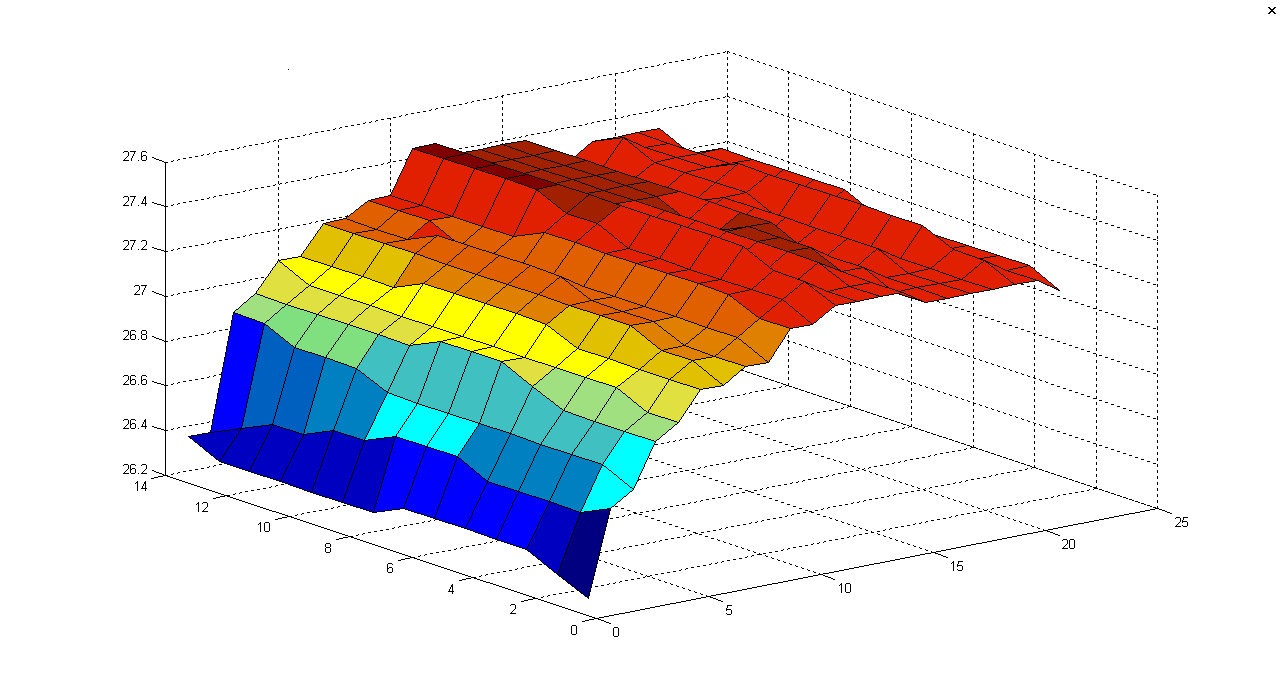
\includegraphics[width=150mm]{img/tempm1.png}
\caption[Temperatur der Zelle]{Temperatur der Zelle}\label{tm1}
\end{figure}

\begin{figure}[htbp]
\centering
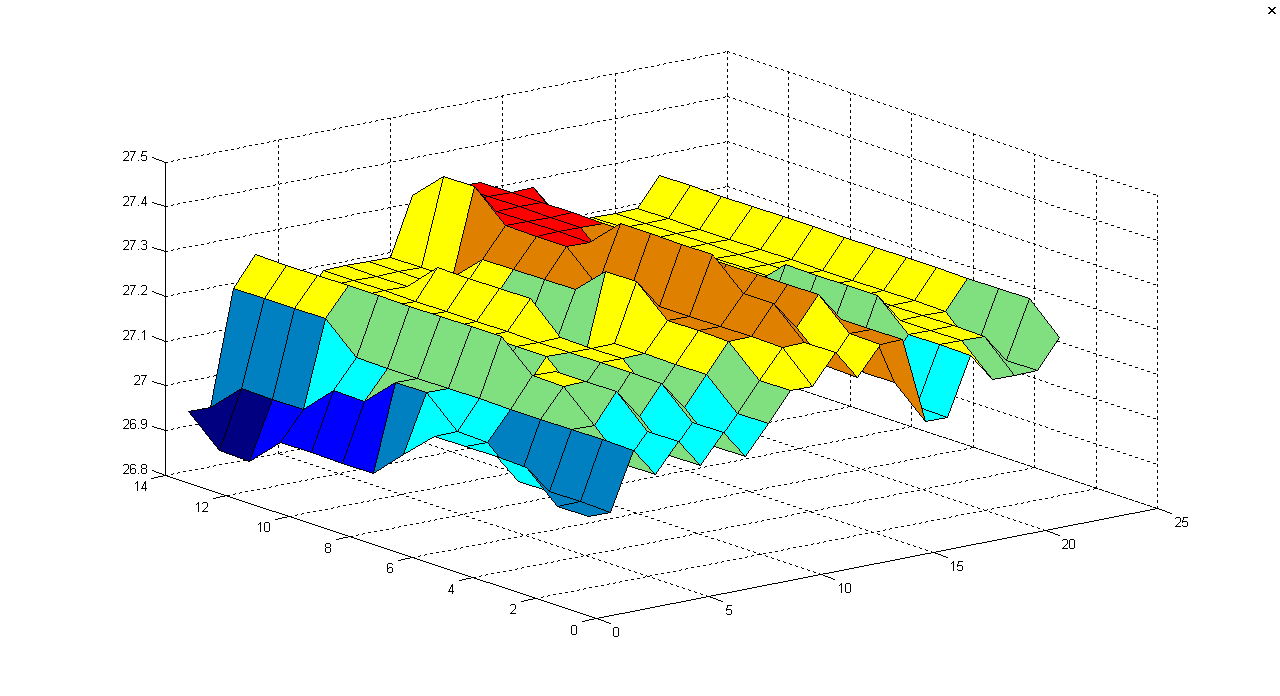
\includegraphics[width=150mm]{img/tempm2.png}
\caption[konstante Temperatur der Zelle]{konstante Temperatur der Zelle}\label{tm2}
\end{figure}


\section{Vermessung der Ausleuchtung einzelner Lampen}

Die geringe Messzeit des Roboters, verglichen mit der mechanischen Methode, macht es möglich die Bestrahlungsstärkeverteilung der einzelnen Lampen in realistischer Zeit zu bestimmen.
Veränderbar sind der Abstand zwischen Lampenfeld und Prüfebene. Die Leistungen der Lampen lassen sich einzeln steuern. 
Die Lampen wurden einzeln mit einer Lampenleistung von 100\% vermessen, die anderen Lampen waren jeweils auf 0\%. Aus den Werten der Einzelmessung wurde optimierte Gesamtausleuchtung errechnet. Diese optimierte Einstellung (welche noch zu messen ist) wird den Herstellerangaben verglichen. Dann wir sich zeigen ob die Methode erfolgsversprechend ist.
Einfacher Algorimus für Matlab:
- Leistung einzelner Lampen nur zwischen 100 und 80%: 
- Eine der mittleren Lampen auf 100\% festsetzen, andere Lampen in einem Bereich von 80\% bis 100\% varieren lassen. Nicht alle Lampen alle 20 Schritte machen lassen. 20 hoch 9 wären sehr viele Rechenschritte.

Zuerst muss eine Lampe bei verschiedenen Einstellungen (100, 90, 80 \%) gemessen werden, um den Zusammenhang von Einstellung der Lampenleistung mit der gemessenen Bestrahlungsstärke zu ermitteln.

\begin{figure}
    \subfigure[3D Ansicht]{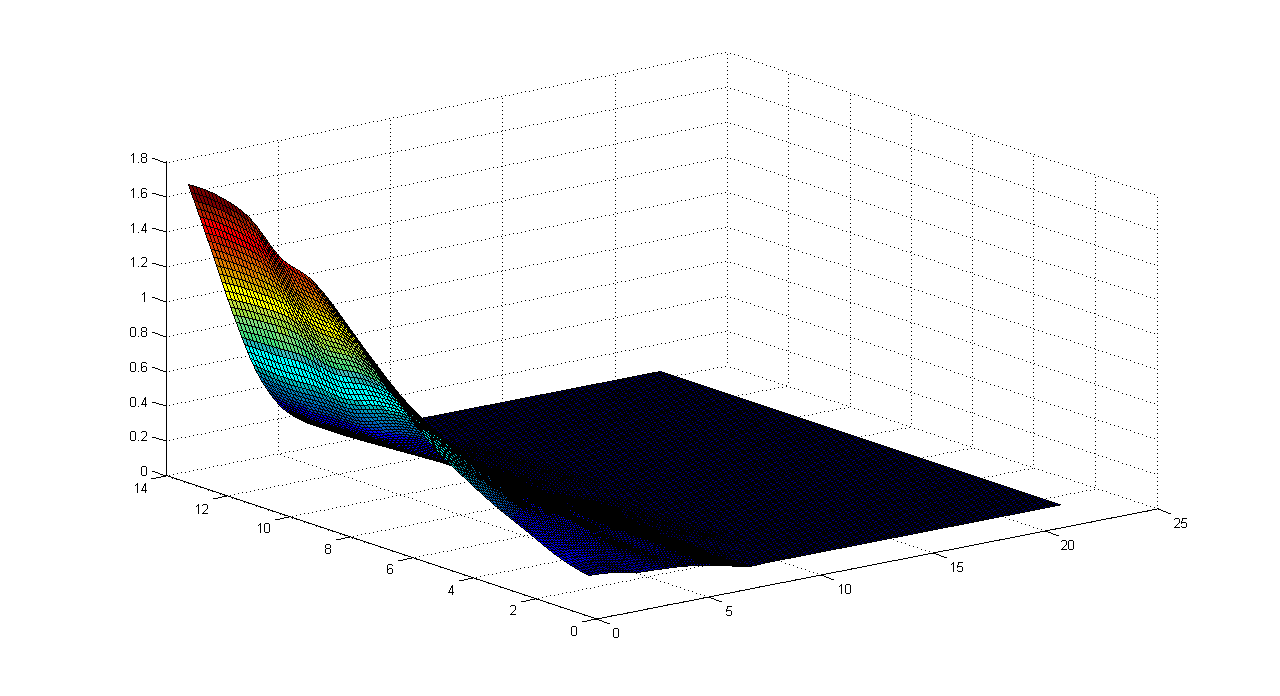
\includegraphics[width=0.49\textwidth]{img/E1.png}}
    \subfigure[Landkarte]{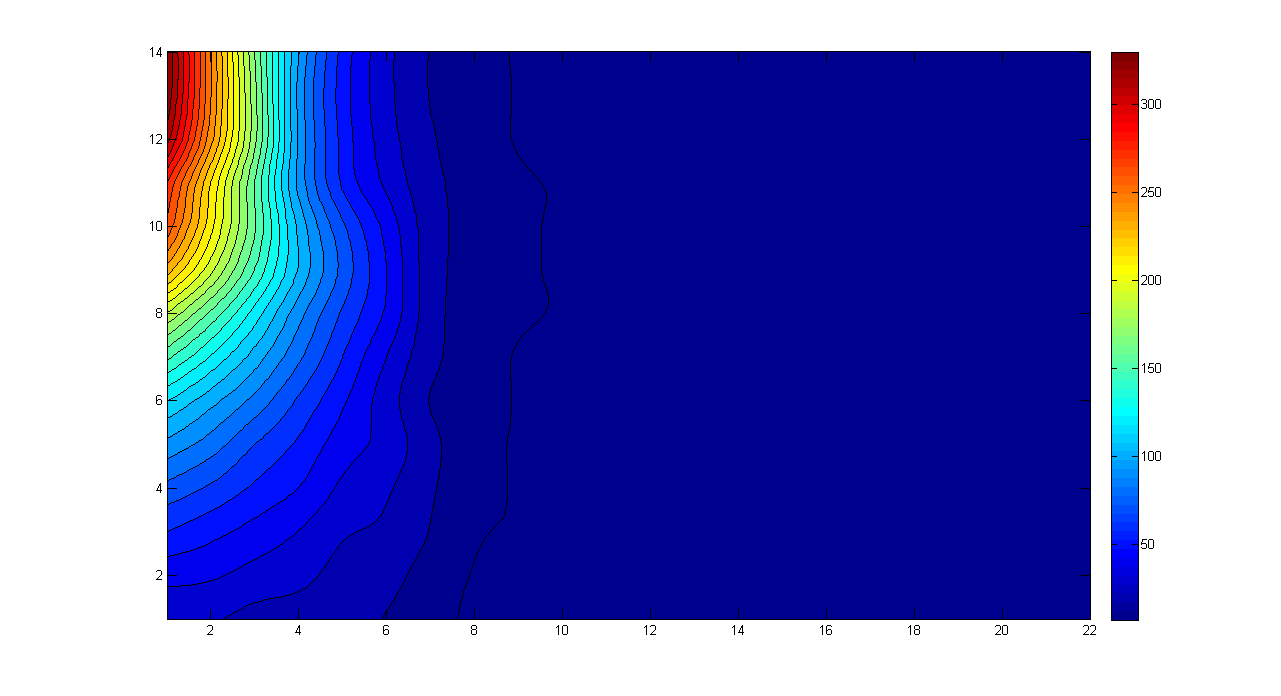
\includegraphics[width=0.49\textwidth]{img/E1a.png}}
\caption{Lampe E1}
\end{figure} 

\begin{figure}
    \subfigure[3D Ansicht]{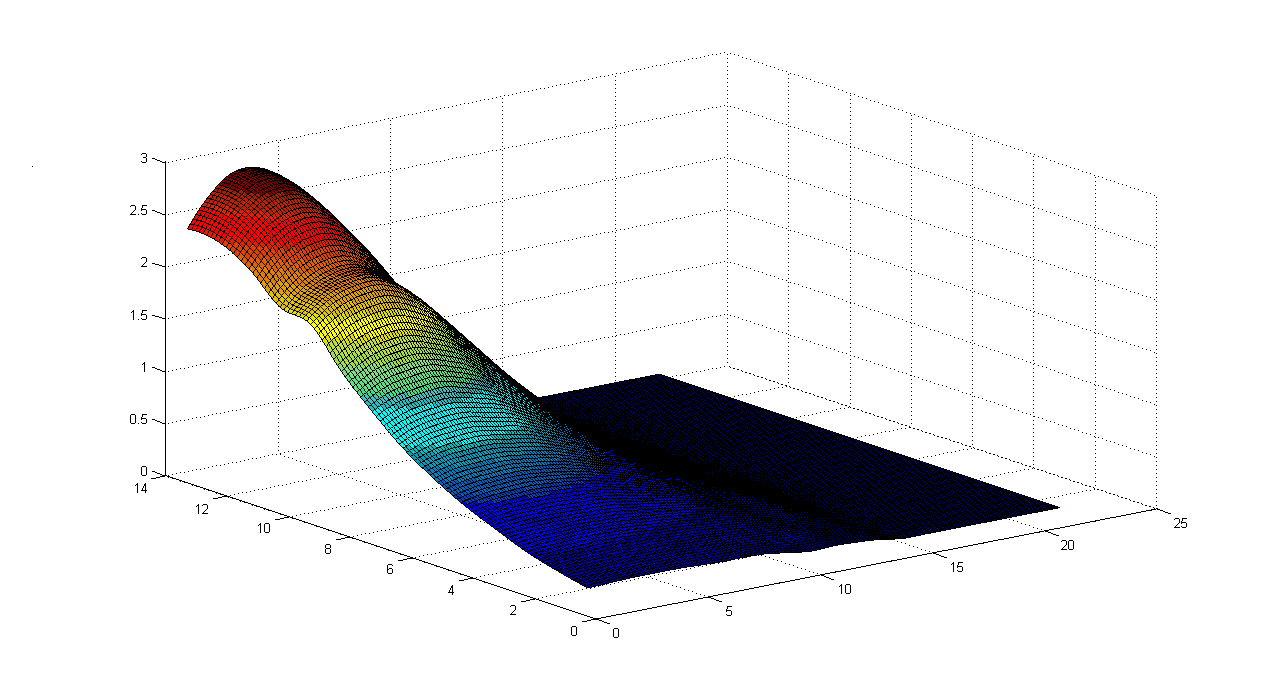
\includegraphics[width=0.49\textwidth]{img/E2.png}}
    \subfigure[Landkarte]{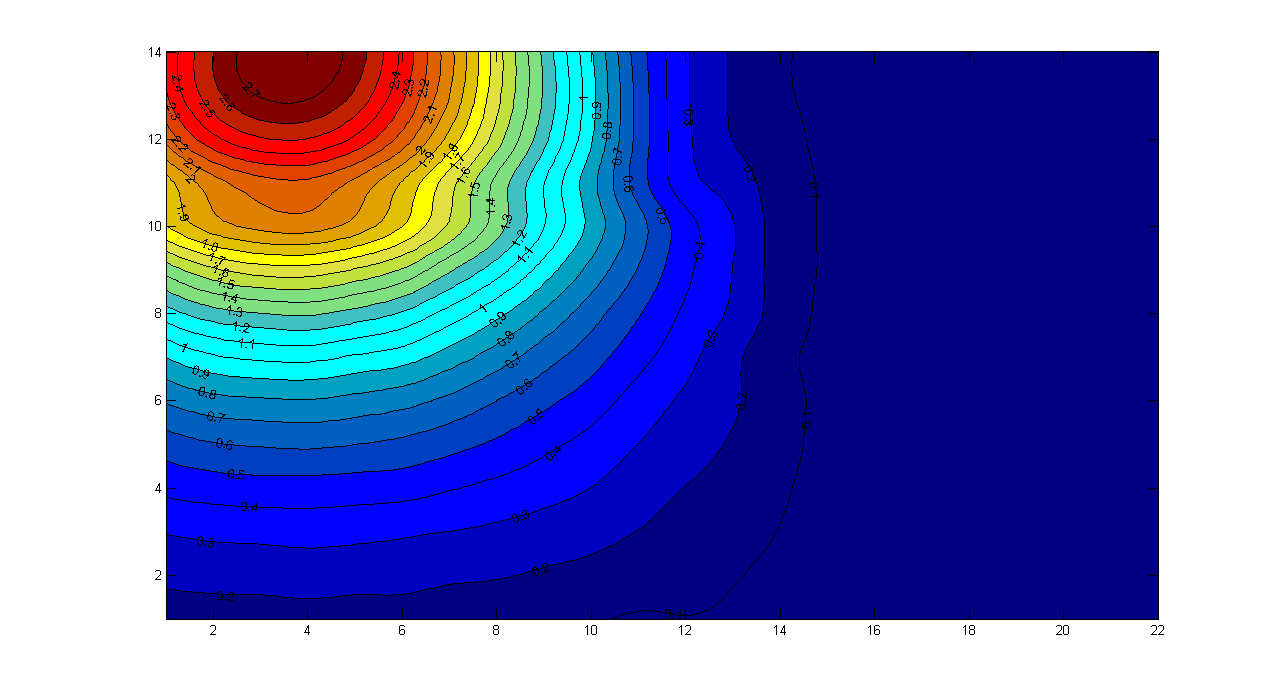
\includegraphics[width=0.49\textwidth]{img/E2a.png}}
\caption{Lampe E2}
\end{figure} 

\begin{figure}
    \subfigure[3D Ansicht]{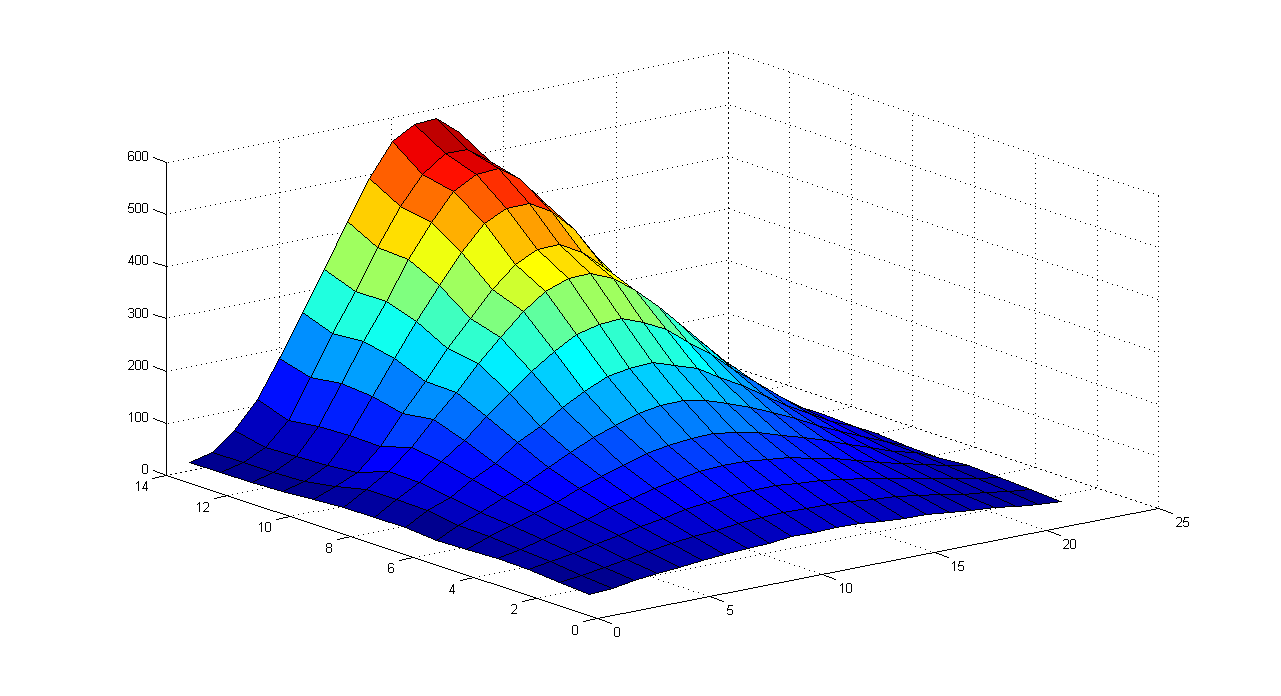
\includegraphics[width=0.49\textwidth]{img/E3.png}}
    \subfigure[Landkarte]{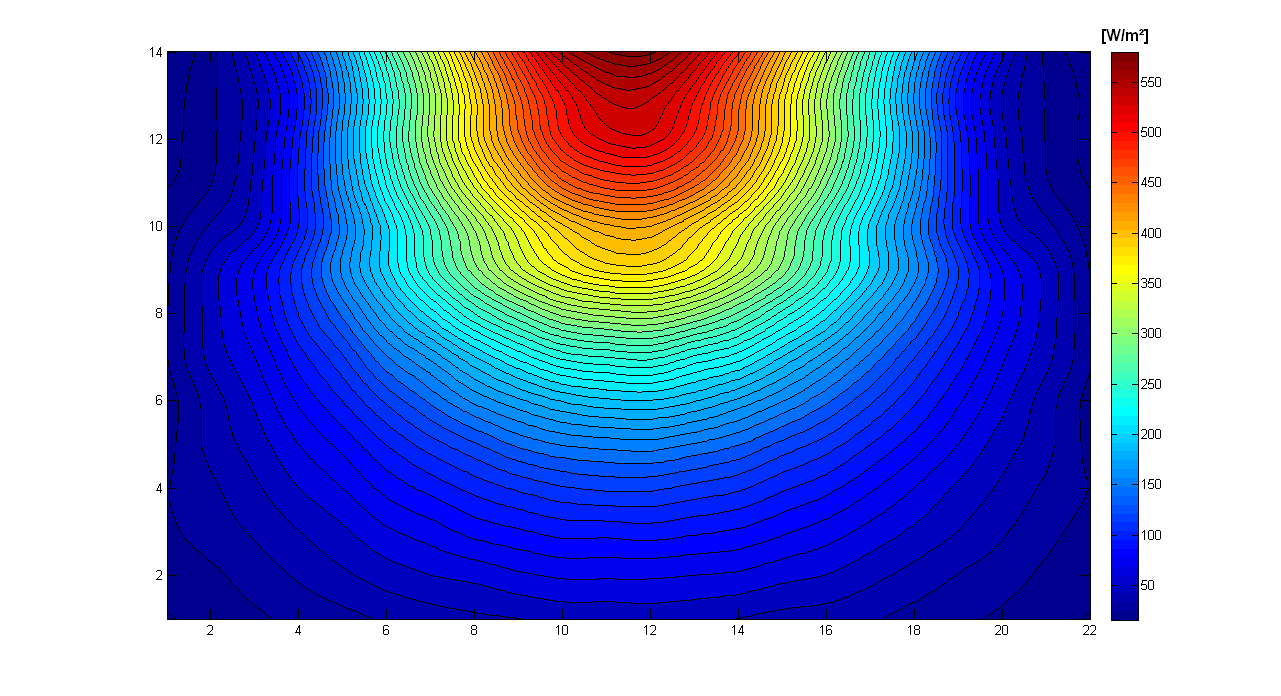
\includegraphics[width=0.49\textwidth]{img/E3a.png}}
\caption{Lampe E3}
\end{figure}

\begin{figure}
    \subfigure[3D Ansicht]{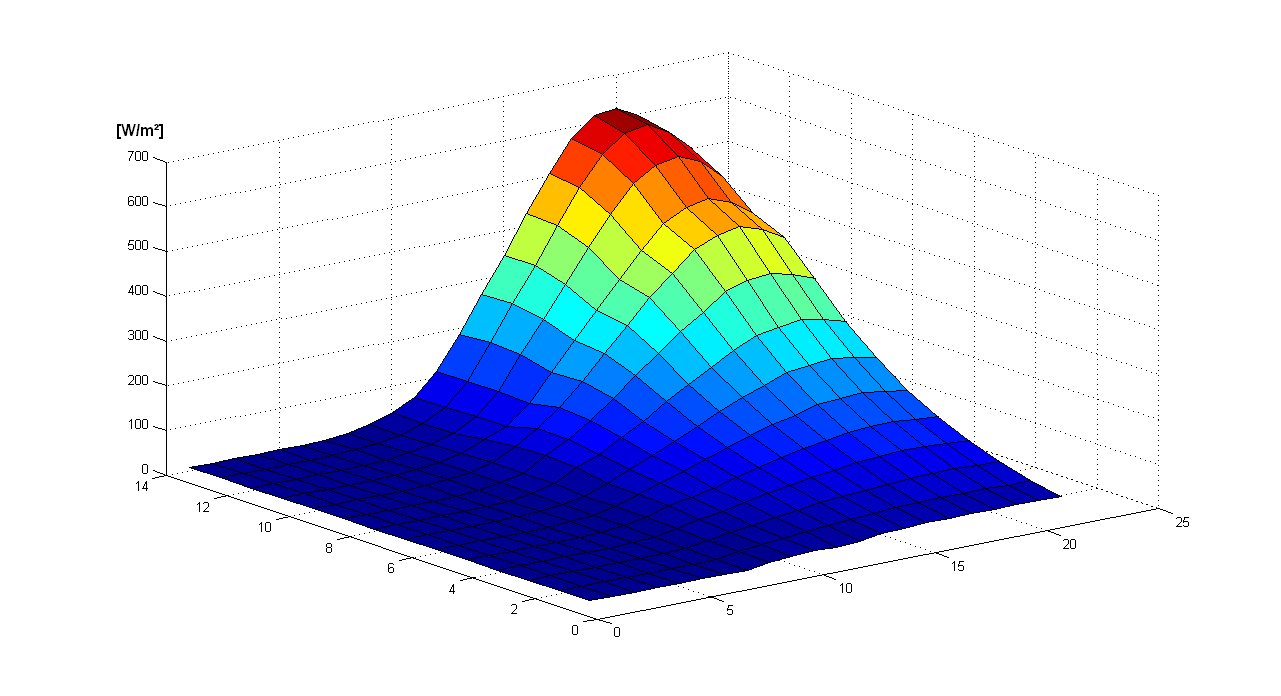
\includegraphics[width=0.49\textwidth]{img/E4.png}}
    \subfigure[Landkarte]{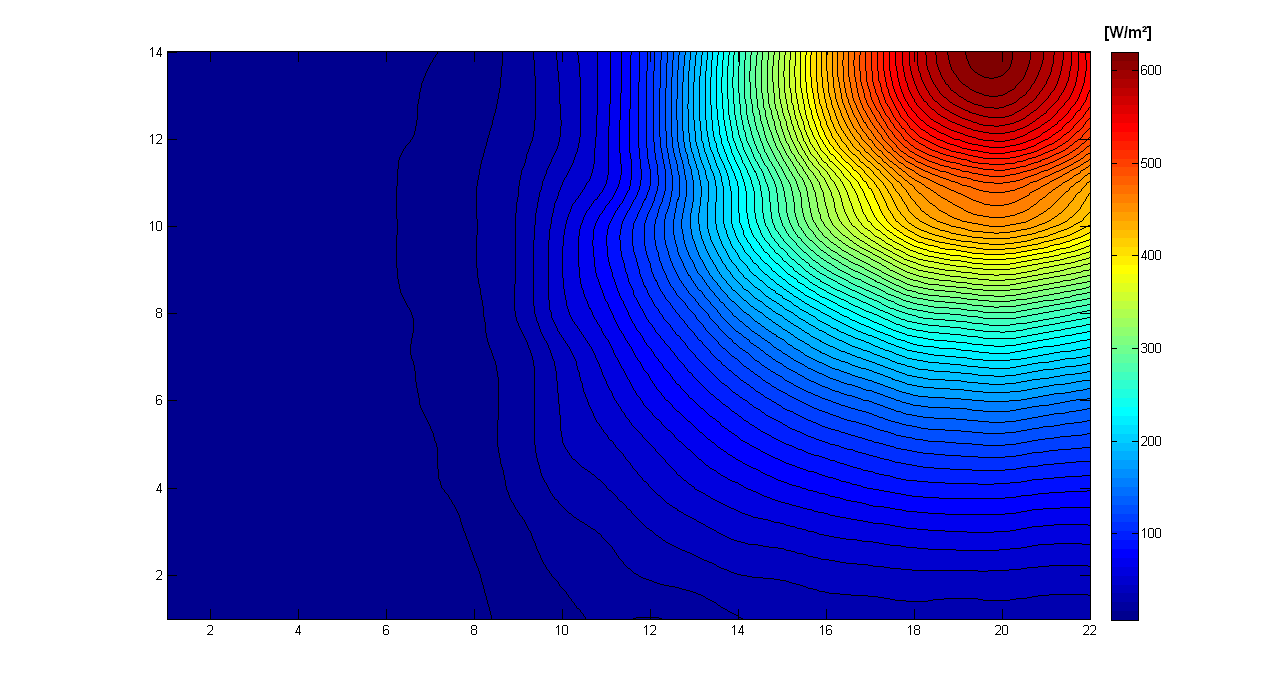
\includegraphics[width=0.49\textwidth]{img/E4a.png}}
\caption{Lampe E4}
\end{figure} 

\begin{figure}
    \subfigure[3D Ansicht]{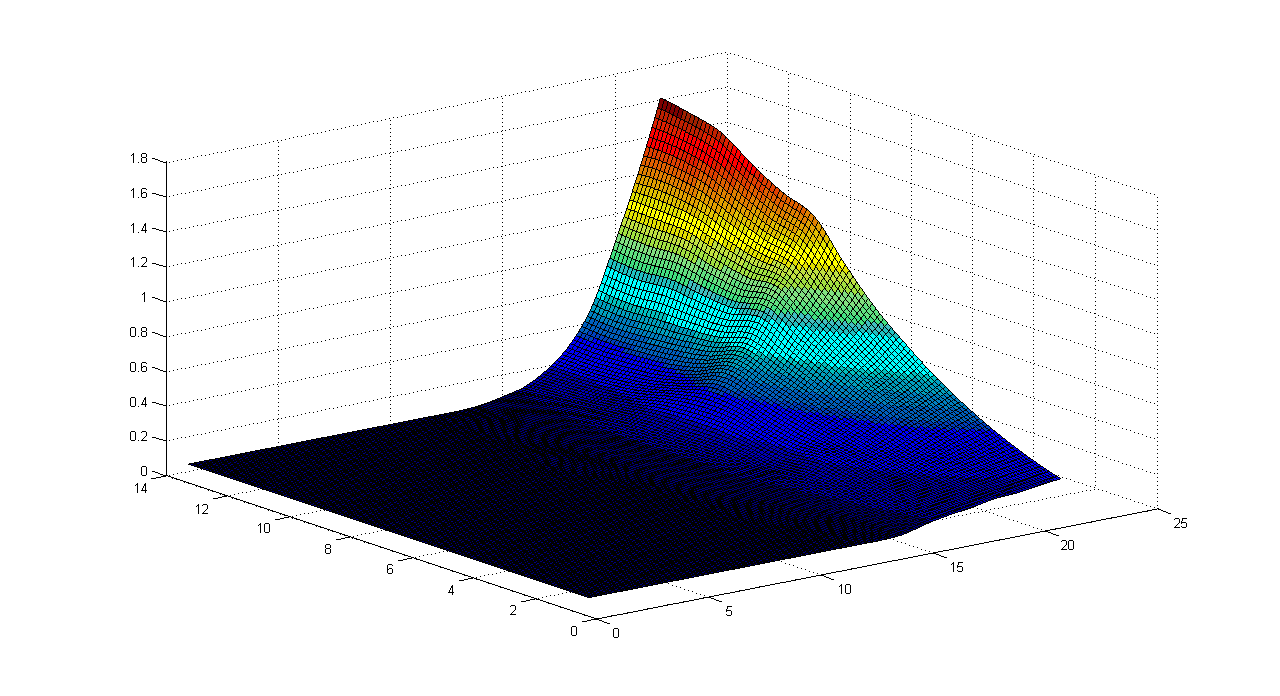
\includegraphics[width=0.49\textwidth]{img/E5.png}}
    \subfigure[Landkarte]{\includegraphics[width=0.49\textwidth]{img/E5a.png}}
\caption{Lampe E5}
\end{figure} 

\begin{figure}
    \subfigure[3D Ansicht]{\includegraphics[width=0.49\textwidth]{img/E6.png}}
    \subfigure[Landkarte]{\includegraphics[width=0.49\textwidth]{img/E6a.png}}
\caption{Lampe E6}
\end{figure} 

\begin{figure}
    \subfigure[3D Ansicht]{\includegraphics[width=0.49\textwidth]{img/E7.png}}
    \subfigure[Landkarte]{\includegraphics[width=0.49\textwidth]{img/E7a.png}}
\caption{Lampe E7}
\end{figure} 

\begin{figure}
    \subfigure[3D Ansicht]{\includegraphics[width=0.49\textwidth]{img/E8.png}}
    \subfigure[Landkarte]{\includegraphics[width=0.49\textwidth]{img/E8a.png}}
\caption{Lampe E8}
\end{figure} 

\begin{figure}
    \subfigure[3D Ansicht]{\includegraphics[width=0.49\textwidth]{img/E9.png}}
    \subfigure[Landkarte]{\includegraphics[width=0.49\textwidth]{img/E9a.png}}
\caption{Lampe E9}
\end{figure} 

\begin{figure}
    \subfigure[3D Ansicht]{\includegraphics[width=0.49\textwidth]{img/E10.png}}
    \subfigure[Landkarte]{\includegraphics[width=0.49\textwidth]{img/E10a.png}}
\caption{Lampe E10}
\end{figure} 





 





\section{Schlussfolgerung}\thispagestyle{empty}

Der Roboter erleichtert die Messung der Bestrahlungsstärkemessung enorm. Durch die kurze Messdauer ist es möglich die Bestrahlungsstärke in periodischen Zeitabständen zu vermessen, um so die Alterung der Lampen zu dokumentieren. 
Diese Art von Messroboter kann in jedem stationären Sonnensimulator entsprechender Größe zur Vermessung der Bestrahlungsstärkeverteilung verwendet werden. 
Die Verwendung des Messroboters erlaubt die Bestrahlungsstärkeverteilung einzelner Lampen zu ermitteln.
Ebenso die Bestrahlungsstärkeverteilung bei unterschiedlichen Höhen des Lampenfeldes.


% Literaturverzeichnis
% Das Literaturverzeichnis kann auch nach einem allf"alligen Anhang positiioniert werden (siehe "`Leitfaden f"ur Bachelor- und Diplomarbeiten"', Version 2.0, Abschnitt 2.9).

% M"oglichkeit 1: Erzeugung des Literaturverzeichnisses mit BibTeX:
% Die Quellen sind in der Datei *.bib (hier Literatur.bib) einzugeben. Danach muss diese Vorlage einmal geTeXt werden, dann BibTeX angewendet werden und 
% anschliessend nochmals zweimal geTeXt werden.
% Im Text erfolgt die Zitierung mit dem Anker-Schl"usselwort, z.B. \cite{kop05}.
\bibliographystyle{IEEEtran}
\bibliography{Literatur}

% M"oglichkeit 2: Erzeugung eines Literaturverzeichnisses ohne BibTeX:
%\begin{thebibliography}{99}
%\bibitem[kop05]{kop05}
%H.~Kopka, {\em LaTeX, Band 1: Einf"uhrung}, Pearson Studium, M"unchen, 3.~Auflage, 2005.
%\bibitem[knu98]{knu98}
%F.~Mittelbach, M.~Goossens, J.~Braams, D.~Carlisle, and Ch. Rowley, {\em The LaTeX Companion}, 
%Addison-Wesley, 2nd edition, 2004.
%\end{thebibliography}

% Abbildungsverzeichnis
\listoffigures
\addcontentsline{toc}{chapter}{Abbildungsverzeichnis} % f"ugt den Eintrag "Abbildungsverzeichnis" im Inhaltsverzeichnis hinzu
\newpage

% Tabellenverzeichnis
\listoftables 
\addcontentsline{toc}{chapter}{Tabellenverzeichnis} % f"ugt den Eintrag "Tabellenverzeichnis" im Inhaltsverzeichnis hinzu
\newpage

% Abk"urzungsverzeichnis
% Bei Verwendung der Dokumentklasse "scrartcl" ist der Befehlt \addchap{Abk"urzungsverzeichnis} durch 
% \addsec{Abk"urzungsverzeichnis} zu ersetzen
\addchap{Abk"urzungsverzeichnis}
\hspace{-17mm}\begin{tabular}{>{\raggedleft}p{0.2\linewidth} p{0.75\linewidth} p{0.1\linewidth}}
www & World Wide Web \\
URL & Uniform Resource Locator
\end{tabular}


% Anh"ange
\begin{appendix}
\chapter{Sourcecode Arduino}

\begin{verbatim}
/*
Programm zum Steuern des Sonnensimulatormessroboters
 Version 1.0 
 */

#include <SD.h>

void vor(int sped);
void zuruck(int sped);
void left(int sped);
void right(int sped);
void tl(int sped);
void tr(int sped);
void ztl();
void ztr();
void vtl();
void vtr();
void halt(); 

// ADCs zum Auslesen der 3x3 Matrix
const int analogInPin0 = A9;  
const int analogInPin1 = A2;
const int analogInPin2 = A5;
const int analogInPin3 = A8;
const int analogInPin4 = A1;
const int analogInPin5 = A4;
const int analogInPin6 = A7;
const int analogInPin7 = A0;
const int analogInPin8 = A3;
const int analogInPin9 = A6;

// Ausgang zum Schalten der Infrarot-Leds
const int analogInPin10 = A10;

// ADC für Messwerte
const int analogInPin12 = A12;
const int analogInPin13 = A13;
const int analogInPin14 = A14;
const int analogInPin15 = A15;

// Digitalausg"ange zum Ansteuern der Motoren
int IN1M1 = 2;
int IN2M1 = 3;
int IN1M2 = 4;
int IN2M2 = 5;
int IN1M3 = 6;
int IN2M3 = 9;
int IN1M4 = 7;
int IN2M4 = 8;

// Sensorwerte der optischen Sensoren (beleuchtet)
int sensorValue0 = 0;        // value read from the pot
int sensorValue1 = 0;        // value read from the pot
int sensorValue2 = 0;        // value read from the pot
int sensorValue3 = 0;        // value read from the pot
int sensorValue4 = 0;        // value read from the pot
int sensorValue5 = 0;        // value read from the pot
int sensorValue6 = 0;        // value read from the pot
int sensorValue7 = 0;        // value read from the pot
int sensorValue8 = 0;        // value read from the pot
int sensorValue9 = 0;        // value read from the pot

// Sensorwerte der optischen Sensoren (unbeleuchtet)
int sensorValue0d = 0;        // value read from the pot
int sensorValue1d = 0;        // value read from the pot
int sensorValue2d = 0;        // value read from the pot
int sensorValue3d = 0;        // value read from the pot
int sensorValue4d = 0;        // value read from the pot
int sensorValue5d = 0;        // value read from the pot
int sensorValue6d = 0;        // value read from the pot
int sensorValue7d = 0;        // value read from the pot
int sensorValue8d = 0;        // value read from the pot
int sensorValue9d = 0;        // value read from the pot

// für Auswertung der opischen Sensoren
int A = 0;
int B = 0;
int C = 0;
int D = 0;
int E = 0;
int F = 0;
int G = 0;
int H = 0;
int I = 0;
int S = 0;

// Grenzwerte für hell (=white) und dunkel (=bleak)
int white = 400;
int white2 = 250;
int bleak = 100;
int bleak2 = 150;

// zur Berechnung der Lage der LInie
float x1,x2,x3,d,k;
float y1,y2,y3,d2,k2;

// einige Hilfsvariablen
char mode='s';
char richtung='v';
int _stop=0;
int vor_ein=0;
int zuruck_ein=0;

// für die Auswertung der Messwerte
long int  temp_modul = 0; 
long int temp_i=0;
long int _Isc = 0; 
long int time = 0; 

// zur Schreiben auf die SD Karte
const int chipSelect = 53;

// Z"ahlvariable für Messpunkt, Spalte und Reihe
int count = 0;
int count2 = 0;
int row = 1;

// zur Schreiben auf die SD Karte
String dataString = "";

// notwendig für die Kommunikation mit SD Karte
void setup() {
  pinMode(A10, OUTPUT);
  pinMode(53, OUTPUT);
  SD.begin(chipSelect);
}

// Definiert alle möglichen Bewegungen
void zuruck(int sped)  
{
  analogWrite(IN1M1,0);
  analogWrite(IN2M1,sped);   
  analogWrite(IN1M2,0);
  analogWrite(IN2M2,sped); 
  analogWrite(IN1M3,0);
  analogWrite(IN2M3,sped); 
  analogWrite(IN1M4,0);
  analogWrite(IN2M4,sped);
}  

void vor(int sped)  
{
  analogWrite(IN1M1,sped);
  analogWrite(IN2M1,0);   
  analogWrite(IN1M2,sped);
  analogWrite(IN2M2,0); 
  analogWrite(IN1M3,sped);
  analogWrite(IN2M3,0); 
  analogWrite(IN1M4,sped);
  analogWrite(IN2M4,0);
}

void left(int sped)  
{
  analogWrite(IN1M1,0);
  analogWrite(IN2M1,sped);   
  analogWrite(IN1M2,sped);
  analogWrite(IN2M2,0); 
  analogWrite(IN1M3,sped);
  analogWrite(IN2M3,0); 
  analogWrite(IN1M4,0);
  analogWrite(IN2M4,sped);
}

void right(int sped)  
{
  analogWrite(IN1M1,sped);
  analogWrite(IN2M1,0);   
  analogWrite(IN1M2,0);
  analogWrite(IN2M2,sped); 
  analogWrite(IN1M3,0);
  analogWrite(IN2M3,sped); 
  analogWrite(IN1M4,sped);
  analogWrite(IN2M4,0);
}

void tr(int sped)
{
  analogWrite(IN1M1,sped);
  analogWrite(IN2M1,0);   
  analogWrite(IN1M2,0);
  analogWrite(IN2M2,sped); 
  analogWrite(IN1M3,sped);
  analogWrite(IN2M3,0); 
  analogWrite(IN1M4,0);
  analogWrite(IN2M4,sped);
}

void tl(int sped)
{
  analogWrite(IN1M1,0);
  analogWrite(IN2M1,sped);   
  analogWrite(IN1M2,sped);
  analogWrite(IN2M2,0); 
  analogWrite(IN1M3,0);
  analogWrite(IN2M3,sped); 
  analogWrite(IN1M4,sped);
  analogWrite(IN2M4,0);
}

void vtr()
{   
  analogWrite(IN1M1,64);
  analogWrite(IN2M1,0);   
  analogWrite(IN1M2,0);
  analogWrite(IN2M2,64); 
  analogWrite(IN1M3,128);
  analogWrite(IN2M3,0); 
  analogWrite(IN1M4,128);
  analogWrite(IN2M4,0);
}

void vtl()
{   
  analogWrite(IN1M1,0);
  analogWrite(IN2M1,64);   
  analogWrite(IN1M2,64);
  analogWrite(IN2M2,0); 
  analogWrite(IN1M3,128);
  analogWrite(IN2M3,0); 
  analogWrite(IN1M4,128);
  analogWrite(IN2M4,0);
}

void ztr()  
{
  analogWrite(IN1M1,0);
  analogWrite(IN2M1,64);   
  analogWrite(IN1M2,0);
  analogWrite(IN2M2,64); 
  analogWrite(IN1M3,0);
  analogWrite(IN2M3,64); 
  analogWrite(IN1M4,64);
  analogWrite(IN2M4,0);
}  

void ztl()  
{
  analogWrite(IN1M1,0);
  analogWrite(IN2M1,64);   
  analogWrite(IN1M2,0);
  analogWrite(IN2M2,64); 
  analogWrite(IN1M3,64);
  analogWrite(IN2M3,0); 
  analogWrite(IN1M4,0);
  analogWrite(IN2M4,64);
}  

void halt()  
{
  analogWrite(IN1M1,0);
  analogWrite(IN2M1,0);   
  analogWrite(IN1M2,0);
  analogWrite(IN2M2,0); 
  analogWrite(IN1M3,0);
  analogWrite(IN2M3,0); 
  analogWrite(IN1M4,0);
  analogWrite(IN2M4,0);
}


// Hauptschleife
void loop() 
{

  // Werte ohne Beleuchtung:
  sensorValue0d = analogRead(analogInPin0);   
  sensorValue1d = analogRead(analogInPin1);  
  sensorValue2d = analogRead(analogInPin2);  
  sensorValue3d = analogRead(analogInPin3);  
  sensorValue4d = analogRead(analogInPin4);  
  sensorValue5d = analogRead(analogInPin5);  
  sensorValue6d = analogRead(analogInPin6);  
  sensorValue7d = analogRead(analogInPin7);  
  sensorValue8d = analogRead(analogInPin8);  
  sensorValue9d = analogRead(analogInPin9);  
  digitalWrite(A10, HIGH);  // LED ein
  delay(2); 
  // Werte mit Beleuchtung:
  sensorValue0 = analogRead(analogInPin0);   
  sensorValue1 = analogRead(analogInPin1);  
  sensorValue2 = analogRead(analogInPin2);  
  sensorValue3 = analogRead(analogInPin3);  
  sensorValue4 = analogRead(analogInPin4);  
  sensorValue5 = analogRead(analogInPin5);  
  sensorValue6 = analogRead(analogInPin6);  
  sensorValue7 = analogRead(analogInPin7);  
  sensorValue8 = analogRead(analogInPin8);  
  sensorValue9 = analogRead(analogInPin9);  
  digitalWrite(A10, LOW);

  A = sensorValue1 - sensorValue1d;
  B = sensorValue2 - sensorValue2d;
  C = sensorValue3 - sensorValue3d;
  D = sensorValue4 - sensorValue4d;
  E = sensorValue5 - sensorValue5d;
  F = sensorValue6 - sensorValue6d;
  G = sensorValue7 - sensorValue7d;
  H = sensorValue8 - sensorValue8d;
  I = sensorValue9 - sensorValue9d;

  S = sensorValue0 - sensorValue0d;

  // zum Erkennen der Linie bei vor- oder zurückfahren 
  x1 = ((C-A)/float(2*A-4*B+2*C));
  x2 = ((F-D)/float(2*D-4*E+2*F));
  x3 = ((I-G)/float(2*G-4*H+2*I));

  d = (x1 + x2 + x3)/3.; // ~ Abstand von der Ideallinie
  k = (x1-x3)/2.;  // Steigung = Verdrehung

  // zum Erkennen der Linie bei links- oder rechtsfahren
  y1 = ((G-A)/float(2*A-4*D+2*G));
  y2 = ((H-B)/float(2*B-4*E+2*H));
  y3 = ((I-C)/float(2*C-4*F+2*I));

  d2 = (y1+y2+y3)/3.;
  k2 = (y3-y1)/2.;

  if( S < bleak2) _stop=0;

  halt();

  if(E>bleak2)
  {

    switch(mode)
    {
    case 's':     // Start
      { 
        halt();
        delay(60000);  // 1 Minuten warten
        mode='v';
      }
      break;

      // Messmode
    case 'e':   // Ende
      {
        halt();
      }
      break;

    case 'm':   // Messen
      { 
        count = count + 1;  // Anzahl der Haltepunkte
        count2 = count2 + 1; 
        dataString = "";
        _stop=1;
        halt();

        delay(250);   // damit die Str"ome der Fahrmotoren keinen Einfluss auf die AD-Wandlung haben

        _Isc = 0;
        temp_modul = 0;
        temp_i = 0;

        // Mittelung über jeweils 500 Messwerte
        for(int i = 0; i < 500 ; i++)
        {
          _Isc = _Isc + analogRead(analogInPin13);  
          temp_modul = temp_modul + analogRead(analogInPin12); 
          temp_i =  temp_i + analogRead(analogInPin15); 
        }
        _Isc = int(_Isc/500.0);
        temp_modul = int(temp_modul/500.0);
        temp_i = int(temp_i/500.0);
        time = millis();

        // Schreiben aud SD-Karte
        dataString += String(time);
        dataString += "\t"; 
        dataString += String(_Isc); 
        dataString += "\t"; 
        dataString += String(temp_modul); 
        dataString += "\t"; 
        dataString += String(temp_i); 
        dataString += "\t"; 
        dataString += String(count); 
        dataString += "\t"; 
        dataString += String(count2); 
        dataString += "\t"; 
        dataString += String(row); 

        // Schreibe aud SD Card
        File dataFile = SD.open("datalog.txt", FILE_WRITE);
        if (dataFile) {
          dataFile.println(dataString);
          dataFile.close();
        }

        // zurück in den Bewegungsmode
        if(richtung=='v') mode='v';
        if(richtung=='z') mode='z';

      }
      break;

    case 'v':   // Vorwärtsfahren
      { 

        richtung='v';

        if(d>0.02)  vtr();
        else 
        {  
          if(d>-0.02)  vor(128);
          else 
            vtl();
        }

        //if((C<bleak)&&(A<bleak))
        if(A<bleak2)
        {
          if(k>0.01) tr(64);
          else
          {
            if(k<-0.01) tl(64);
          }

          if(d>0.025) right(64);
          else
          {
            if(d<-0.025) left(64);
          }
        }   
        if((A>white)&&(B>white)) mode='a'; 

        if((_stop==0)&&(S>white2)) mode='m';   


      }
      break;

    case 'z': // Rückwärtsfahren
      { 

        richtung='z';

        if(d>0.02)  ztr();
        else 
        {  
          if(d>-0.02)  zuruck(128);
          else  ztl();
        }

        //if((G<bleak)&&(I<bleak))
        if(G<bleak2)
        {
          if(k>0.01) tr(64);
          else
          {
            if(k<-0.01) tl(64);
          }

          if(d>0.025) right(64);
          else
          {
            if(d<-0.025) left(64);
          }
        }
        if((G>white)&&(H>white)) mode='c';

        if((_stop==0)&&(S>white2)) mode='m';  

        if((I<bleak)&&(H<bleak)&&(G<bleak)) mode='e';

      }
      break; 

    case 'r':     //nach rechts
      {
        richtung='r';
        count2 = 0;

        right(128);
        if(D>white2)
        {
          if(d2>0.04) vor_ein=1;
          if(d2<0.02) vor_ein=0;
          if(d2<-0.04) zuruck_ein=1;
          if(d2>-0.02) zuruck_ein=0;

          if(vor_ein==1) vor(64);
          if(zuruck_ein==1) zuruck(64);

          if((vor_ein==0)&&(zuruck_ein==0))
          {
            if(k2>0.02) tr(64);
            else
            {
              if(k2<-0.02) tl(64);
            }
          }
        }

        if((D<bleak)&&(G<bleak)&&(A<bleak)) 
        { 
          mode='b';
        }

      } 
      break;

    case 'l':    // auch nach rechts 
      {
        richtung=='l';
        count2 = 0;

        right(128);
        //if((C<bleak)&&(I<bleak))
        if(D>white2)
        {
          if(d2>0.04) vor_ein=1;
          if(d2<0.02) vor_ein=0;
          if(d2<-0.04) zuruck_ein=1;
          if(d2>-0.02) zuruck_ein=0;

          if(vor_ein==1) vor(64);
          if(zuruck_ein==1) zuruck(64);

          if((vor_ein==0)&&(zuruck_ein==0))
          {
            if(k2>0.02) tr(64);
            else
            {
              if(k2<-0.02) tl(64);
            }
          }
        }

        if((D<bleak)&&(G<bleak)&&(A<bleak))
        { 
          mode='d';
        }

      } 
      break;

    case 'a':  // Um die Ecke fahren
      {
        if((A>bleak2)&&(B>bleak2)) vor(64);
        else 
        { 
          right(64);
          delay(700);
          halt();
          row = row +1 ;

          mode='r';

        }
      } 
      break; 

    case 'b':  // Um die Ecke fahren
      {

        zuruck(64);
        delay(850);
        halt();
        delay(500);

        mode='x';

      } 
      break; 

    case 'x':
      {
        if(d>0.025) right(64);

        if(d<-0.025) left(64);

        if((d<0.1)&&(d>-0.1)) mode='y';
      }
      break;

    case 'y':
      {
        if(k>0.01) tr(32);

        if(k<-0.01) tl(32);

        if((k<0.04)&&(k>-0.04)) mode='z';
      }
      break;

    case 'c':  // Um die Ecke fahren
      {
        if((H>bleak2)&&(G>bleak2 )) zuruck(64);
        else 
        { 
          right(64);
          delay(700);
          halt();
          row = row +1 ;

          mode='l';
        }
      } 
      break; 

    case 'd':  // Um die Ecke fahren
      {

        vor(64);
        delay(850);
        halt();
        delay(500);
        mode='q';

      } 
      break; 

    case 'q':
      {
        if(d>0.025) right(64);

        if(d<-0.025) left(64);

        if((d<0.1)&&(d>-0.1))       mode='p';
      }
      break;


    case 'p':
      {
        if(k>0.01) tr(32);

        if(k<-0.01) tl(32);

        if((k<0.04)&&(k>-0.04)) mode='v'; 

      }
      break;
    } 
  }   


  else 
  {  
    if((richtung=='v')||(richtung=='z'))
    {
      if((A>bleak2)||(D>bleak2)||(G>bleak2)||(C>bleak2)||(F>bleak2)||(I>bleak2))
      {
        if((A+D+G)>(C+F+I)) right(128);
        else left(128);
      }
      else halt();
    }


    if((richtung=='r')||(richtung=='l'))
    {
      if((A>bleak2)||(B>bleak2)||(C>bleak2)||(G>bleak2)||(H>bleak2)||(I>bleak2))
      {
        if((A+B+C)>(G+H+I)) vor(64);
        else zuruck(64);
      }
      else halt();
    }
  }

  delay(5); 

}
\end{verbatim}

\chapter{Sourcecode Auswertung}



\begin{verbatim}

% Graphische Auswertung der Robotermesswerte

close all;
clc;
clear all;

% "Offnen der Datei, welche eine Messfahrt mit genau 308 Messwerten
% enthalten muss
fid = fopen('data1.txt', 'r');
a = fscanf(fid, '%g %g', [7 308])     
a = a';
fclose(fid)

j=1; k=1; l=1;

% Umwandeln der 1 dimensionalen Modultemperatur ADC-Werte in eine Matrix:
for(i=0:307)
    if(mod(i,28)>13) k = 28- mod(i,28);
    else k = mod(i,14)+1;
    end
    Tm(k,l)=a(i+1,3);
    if(mod(i+1,14)==0) l=l+1;
    end
end

% Umrechnung der ADC-Werte in Temeratur:
Rm = (Tm +4038.9)/40.107;  % ADC --> Widerstand
TTm = (Rm-100.03)/0.3879;  % Widerstand --> Temperatur

j=1; k=1; l=1;

% Umwandeln der 1 dimensionalen Innentemperatur ADC-Werte in eine Matrix:
for(i=0:307)
    if(mod(i,28)>13) k = 28- mod(i,28);
    else k = mod(i,14)+1;
    end
    Ti(k,l)=a(i+1,4);
    if(mod(i+1,14)==0) l=l+1;
    end
end

% Umrechnung der ADC-Werte in Temeratur:
Ri = (Ti +4023.6)/40.027;  % ADC --> Widerstand
TTi = (Ri-100.03)/0.3879;  % Widerstand --> Temperatur

j=1; k=1; l=1;

% Umwandeln der 1 dimensionalen Kurzschlusstrom ADC-Werte in eine Matrix:
for(i=0:307)
    if(mod(i,28)>13) k = 28- mod(i,28);
    else k = mod(i,14)+1;
    end
    I(k,l)=a(i+1,2);
    if(mod(i+1,14)==0) l=l+1;
    end
end

% Umrechnung der ADC-Werte in Ampere:

A = (I +4.5766)/119.2;   % ADC --> Ampere
A = A - (TTm-25)*0.004;  % Temperaturkorrektur



[XI,YI] = meshgrid(1:.125:22, 1:.125:14);

Ai = interp2(A,XI,YI,'cubic'); % Interpolation

A_max = max(max(Ai));
A_min = min(min(Ai));

Normiert = Ai / A_max * 1.1;

w = (A_max - A_min)/(A_max + A_min) * 100  % maximale Abweichung in Protzent

% Graphische Darstellung des Stromes
figure;
surf(XI,YI,Ai);   % in Ampere


% Graphische Darstellung des normierten Stromes
zlevs2 = 0.9:0.01:1.1;
figure;
[C,h] = contourf(XI,YI,Normiert,zlevs2);
set(h,'ShowText','on','TextStep',get(h,'LevelStep')*2)
colorbar;

% Graphische Darstellung der Modultemperatur
figure;
surf(TTm); 

% Graphische Darstellung der Umgebungstemperatur
figure;
surf(TTi);

\end{verbatim} 

\end{appendix}


\end{document}
